% Artigo LNCS — Estudo Comparativo de Metaheurísticas
% Compilar com: pdflatex artigo.tex (duas vezes)
\documentclass[runningheads]{llncs}

\usepackage[T1]{fontenc}
\usepackage[utf8]{inputenc}
\usepackage[brazil]{babel}
\usepackage{graphicx}
\usepackage{amsmath}
\usepackage{amssymb}
\usepackage{booktabs}
\usepackage{multirow}
\usepackage{array}
\usepackage{float}
\usepackage{algorithm}
\usepackage{algpseudocode}
\usepackage{hyperref}
\usepackage[table]{xcolor}
\usepackage{caption}
\usepackage{subcaption}

% Ajuste de largura de coluna para tabelas
\newcolumntype{C}[1]{>{\centering\arraybackslash}p{#1}}

\begin{document}

\title{Estudo Comparativo de Algoritmos Metaheurísticos para
Otimização de Fun\c{c}\~{o}es Benchmark: AG, DE, PSO e EPSO
em M\'{u}ltiplas Dimens\~{o}es}

\titlerunning{Estudo Comparativo de Metaheur\'{i}sticas}

\author{Davi\inst{1}}
\authorrunning{Davi}

\institute{Universidade Federal do Rio de Janeiro (UFRJ), Rio de Janeiro, Brasil\\
\email{aluno@ic.ufrj.br}}

\maketitle

%─────────────────────────────────────────────────────────────────────────────
\begin{abstract}
Este trabalho apresenta um estudo comparativo entre quatro algoritmos
metaheurísticos de otimização contínua: Algoritmo Genético~(AG),
Evolução Diferencial~(DE), Otimização por Enxame de Partículas~(PSO)
e Otimização Evolutiva por Enxame de Partículas~(EPSO). Os algoritmos
são avaliados em dez funções benchmark escaláveis — cinco unimodais e
cinco multimodais — nas dimensões 30, 50 e 100. O protocolo experimental
adota 51~execuções independentes por configuração com um orçamento fixo
de 100.000~avaliações de função. Os hiperparâmetros de cada algoritmo
foram ajustados individualmente por meio do framework Optuna com o
amostrador TPE\@. A comparação estatística segue o método de Marcelino
et al.~\cite{marcelino2018}, com Teste~T independente por par de
algoritmos ao nível de significância de 5\%. Os resultados indicam que
o desempenho relativo dos algoritmos varia significativamente conforme
o tipo de função e a dimensão do problema, evidenciando que nenhum
algoritmo domina em todos os cenários avaliados.

\keywords{Metaheurísticas \and Algoritmo Genético \and Evolução
Diferencial \and PSO \and EPSO \and Funções Benchmark \and Otimização
Contínua}
\end{abstract}

%─────────────────────────────────────────────────────────────────────────────
\section{Introdução}
\label{sec:intro}

Problemas de otimização contínua surgem em diversas áreas da engenharia
e da ciência, muitas vezes caracterizados por espaços de busca de alta
dimensionalidade, não-convexidade e multimodalidade~\cite{storn1997}.
Algoritmos metaheurísticos têm se destacado como alternativas eficazes
aos métodos determinísticos clássicos nesses cenários, uma vez que não
requerem informação de gradiente e são capazes de escapar de ótimos
locais por meio de mecanismos estocásticos de busca.

Dentre os algoritmos mais estudados na literatura, o Algoritmo Genético
(AG) representa o paradigma evolutivo clássico, fundamentado nos
princípios da seleção natural e da genética~\cite{goldberg1989}. A
Evolução Diferencial (DE) surgiu como uma alternativa competitiva
baseada em mutação diferencial e cruzamento binomial, demonstrando
desempenho consistente em funções de benchmark~\cite{storn1997}. O PSO
introduziu o conceito de inteligência coletiva por meio da interação
entre partículas guiadas por memória individual e social~\cite{kennedy1995}.
O EPSO estende o PSO com auto-adaptação dos pesos estratégicos e
perturbação multiplicativa do melhor global, incorporando características
das Estratégias Evolutivas~\cite{miranda2002}.

Apesar do extenso corpo de literatura sobre cada um desses algoritmos
individualmente, comparações sistemáticas que avaliem seu desempenho em
múltiplas funções e dimensões sob um protocolo experimental uniforme
permanecem relevantes, especialmente com técnicas modernas de ajuste de
hiperparâmetros. Este trabalho contribui com uma avaliação comparativa
rigorosa dos quatro algoritmos, utilizando Optuna para otimização
automatizada de hiperparâmetros e análise estatística para validação
das diferenças observadas.

%O restante do artigo está organizado da seguinte forma: a
%Seção~\ref{sec:algoritmos} descreve os quatro algoritmos; a
%Seção~\ref{sec:benchmark} apresenta as funções benchmark; a
%Seção~\ref{sec:metodologia} detalha a metodologia experimental; a
%Seção~\ref{sec:resultados} apresenta e discute os resultados; e a
%Seção~\ref{sec:conclusao} conclui o trabalho.

%─────────────────────────────────────────────────────────────────────────────
\section{Algoritmos}
\label{sec:algoritmos}

\subsection{Algoritmo Genético (AG)}

O Algoritmo Genético é uma metaheurística evolutiva inspirada na teoria
da seleção natural de Darwin~\cite{goldberg1989}. Uma população de
indivíduos evolui ao longo de gerações por meio de três operadores
fundamentais: seleção, cruzamento e mutação.

Na implementação adotada, a \textbf{seleção} utiliza torneio de
tamanho~$k=3$, escolhendo o mais apto entre $k$~indivíduos sorteados
aleatoriamente. O \textbf{cruzamento} emprega o operador BLX-$\alpha$,
que gera um descendente no intervalo estendido $[\min(p_1, p_2) -
\alpha\Delta,\ \max(p_1, p_2) + \alpha\Delta]$, onde $\Delta =
|p_1 - p_2|$. A \textbf{mutação} do tipo \emph{creep} aplica uma
perturbação gaussiana de desvio padrão $\sigma$ a cada gene com
probabilidade $p_m$. A aptidão de toda a nova população é avaliada
de forma vetorizada a cada geração.

\begin{algorithm}[ht]
\caption{Algoritmo Genético (AG)}
\label{alg:ag}
\begin{algorithmic}[1]
\Require $f$, $D$, $(l,u)$, $N$, maxFEs, $k$, $\alpha$, $p_m$, $\sigma$
\State Inicializar $P \leftarrow \mathcal{U}(l,u)^{N \times D}$
\State $\text{fit} \leftarrow f(P)$;\ \ $\text{FEs} \leftarrow N$
\While{$\text{FEs} < \text{maxFEs}$}
  \For{$i = 1$ \textbf{to} $N$}
    \State $p_1 \leftarrow \text{Torneio}(P, \text{fit}, k)$
    \State $p_2 \leftarrow \text{Torneio}(P, \text{fit}, k)$
    \State $o_i \leftarrow \text{BLX-}\alpha(p_1, p_2)$
    \State $o_i \leftarrow \text{CreepMutação}(o_i, p_m, \sigma)$
  \EndFor
  \State $P \leftarrow O$;\ \ $\text{fit} \leftarrow f(P)$
  \State $\text{FEs} \leftarrow \text{FEs} + N$
\EndWhile
\State \Return melhor indivíduo de $P$
\end{algorithmic}
\end{algorithm}

\subsection{Evolução Diferencial (DE)}

A Evolução Diferencial~\cite{storn1997} opera sobre uma população de
vetores reais, gerando candidatos por meio de mutação diferencial e
cruzamento binomial, com seleção \emph{greedy} individual.

A estratégia adotada é DE/rand/1/bin: o vetor mutante é gerado como
$v_i = x_{r_0} + F(x_{r_1} - x_{r_2})$, onde $r_0, r_1, r_2$ são
índices distintos sorteados aleatoriamente e $F$ é o fator de escala.
O cruzamento binomial combina $v_i$ com o vetor alvo $x_i$ gene a
gene com probabilidade CR, garantindo ao menos um gene do mutante por
meio do índice $j_{\text{rand}}$. A seleção substitui $x_i$ pelo
candidato $u_i$ apenas se $f(u_i) \leq f(x_i)$.

\begin{algorithm}[ht]
\caption{Evolução Diferencial (DE/rand/1/bin)}
\label{alg:de}
\begin{algorithmic}[1]
\Require $f$, $D$, $(l,u)$, $N$, maxFEs, $F$, CR
\State Inicializar $P \leftarrow \mathcal{U}(l,u)^{N \times D}$
\State $\text{fit} \leftarrow f(P)$;\ \ $\text{FEs} \leftarrow N$
\While{$\text{FEs} < \text{maxFEs}$}
  \For{$i = 1$ \textbf{to} $N$}
    \State Sortear $r_0, r_1, r_2 \in \{1,\ldots,N\} \setminus \{i\}$
    \State $v_i \leftarrow x_{r_0} + F(x_{r_1} - x_{r_2})$;\ \
           $v_i \leftarrow \text{clip}(v_i, l, u)$
    \State $j_{\text{rand}} \leftarrow \mathcal{U}\{1,\ldots,D\}$
    \For{$j = 1$ \textbf{to} $D$}
      \State $u_{i,j} \leftarrow v_{i,j}$ se $\mathcal{U}(0,1) < \text{CR}$
             ou $j = j_{\text{rand}}$, senão $x_{i,j}$
    \EndFor
    \If{$f(u_i) \leq \text{fit}_i$}
      \State $x_i \leftarrow u_i$;\ \ $\text{fit}_i \leftarrow f(u_i)$
    \EndIf
    \State $\text{FEs} \leftarrow \text{FEs} + 1$
  \EndFor
\EndWhile
\State \Return melhor indivíduo de $P$
\end{algorithmic}
\end{algorithm}

\subsection{Otimização por Enxame de Partículas (PSO)}

O PSO~\cite{kennedy1995} modela um enxame de partículas que se movem
pelo espaço de busca sob influência de três componentes: inércia,
memória individual (\emph{pbest}) e memória social (\emph{gbest}).

A equação de atualização de velocidade é:
\begin{equation}
  v_i^{t+1} = w\,v_i^t
    + c_1 r_1 (p_i^{\text{best}} - x_i^t)
    + c_2 r_2 (g^{\text{best}} - x_i^t),
\end{equation}
onde $w$ é o peso de inércia, $c_1$ e $c_2$ os coeficientes de
aceleração, e $r_1, r_2 \sim \mathcal{U}(0,1)$. A velocidade é
limitada a $v_{\max} = 0{,}2\,(u - l)$ e as posições são projetadas
ao domínio por \emph{clipping}.

\begin{algorithm}[ht]
\caption{Otimização por Enxame de Partículas (PSO)}
\label{alg:pso}
\begin{algorithmic}[1]
\Require $f$, $D$, $(l,u)$, $N$, maxFEs, $w$, $c_1$, $c_2$
\State Inicializar $X \leftarrow \mathcal{U}(l,u)^{N\times D}$,
       $V \leftarrow \mathcal{U}(-v_{\max},v_{\max})^{N\times D}$
\State $\text{fit} \leftarrow f(X)$;\ \ $\text{pbest} \leftarrow X$;
       $g^{\text{best}} \leftarrow \arg\min \text{fit}$
\State $\text{FEs} \leftarrow N$
\While{$\text{FEs} < \text{maxFEs}$}
  \For{$i = 1$ \textbf{to} $N$}
    \State $V_i \leftarrow w V_i + c_1 r_1(p_i^{\text{best}}-X_i)
           + c_2 r_2(g^{\text{best}}-X_i)$
    \State $V_i \leftarrow \text{clip}(V_i,-v_{\max},v_{\max})$
    \State $X_i \leftarrow \text{clip}(X_i + V_i, l, u)$
    \State $\text{fit}_i \leftarrow f(X_i)$;\ \
           $\text{FEs} \leftarrow \text{FEs}+1$
    \If{$\text{fit}_i < f(p_i^{\text{best}})$}
      \State $p_i^{\text{best}} \leftarrow X_i$
      \If{$\text{fit}_i < f(g^{\text{best}})$}
        \State $g^{\text{best}} \leftarrow X_i$
      \EndIf
    \EndIf
  \EndFor
\EndWhile
\State \Return $g^{\text{best}}$
\end{algorithmic}
\end{algorithm}

\subsection{Otimização Evolutiva por Enxame de Partículas (EPSO)}

O EPSO~\cite{miranda2002} estende o PSO incorporando auto-adaptação
dos pesos estratégicos e seleção \emph{greedy} entre cada partícula e
seu clone. Para cada partícula $i$, um clone herda os pesos mutados
por ruído gaussiano:
\begin{equation}
  w_j^* = w_j + \tau\,\mathcal{N}(0,1), \quad w_j^* \in [0,1].
\end{equation}
O melhor global é perturbado multiplicativamente antes do movimento:
\begin{equation}
  g_j^* = g_j\,(1 + w_{\text{pert}}\,\xi), \quad \xi \sim \mathcal{U}(0,1),
\end{equation}
aplicado apenas às dimensões selecionadas pela máscara de comunicação
estocástica com probabilidade $p_c$ por dimensão. A seleção mantém o
indivíduo (original ou clone) com menor aptidão.

\begin{algorithm}[H]
\small
\caption{Otimização Evolutiva por Enxame de Partículas (EPSO)}
\label{alg:epso}
\begin{algorithmic}[1]
\Require $f$, $D$, $(l,u)$, $N$, maxFEs, $\tau$, $p_c$
\State Inicializar $X$, $V$, pesos $W \in [0,1]^{N\times 4}$, pbest, gbest
\State $\text{FEs} \leftarrow N$
\While{$\text{FEs} < \text{maxFEs}$}
  \For{$i = 1$ \textbf{to} $N$}
    \State $W_i^* \leftarrow \text{clip}(W_i + \tau\,\mathcal{N}(0,1)^4,\,0,1)$
    \State $g^* \leftarrow \text{PerturbGbest}(g^{\text{best}}, W_i^*, p_c)$
    \State $V_i^{\text{clone}} \leftarrow W_{i,\text{iner}}^*\,V_i
           + W_{i,\text{mem}}^*\,r_1(p_i^{\text{best}}-X_i)
           + W_{i,\text{coop}}^*\,r_2\,C(g^*-X_i)$
    \State $X_i^{\text{clone}} \leftarrow \text{clip}(X_i+V_i^{\text{clone}},l,u)$
    \State Mover original com $W_i$; avaliar original e clone; $\text{FEs} \leftarrow \text{FEs}+2$
    \If{$f(X_i^{\text{clone}}) < f(X_i^{\text{orig}})$}
      \State $X_i \leftarrow X_i^{\text{clone}}$; $W_i \leftarrow W_i^*$
    \Else
      \State $X_i \leftarrow X_i^{\text{orig}}$
    \EndIf
    \State Atualizar pbest e gbest
  \EndFor
\EndWhile
\State \Return $g^{\text{best}}$
\end{algorithmic}
\end{algorithm}

%─────────────────────────────────────────────────────────────────────────────
\section{Fun\c{c}\~{o}es Benchmark}
\label{sec:benchmark}

As dez funções selecionadas cobrem diferentes características de
dificuldade: separabilidade, multimodalidade, não-separabilidade,
condicionamento e deceptividade.

\subsection{Fun\c{c}\~{o}es Unimodais}

\subsubsection{Sphere}\leavevmode
$f(\mathbf{x}) = \sum_{i=1}^{D} x_i^2$, domínio $[-100,\,100]^D$.
Separável e convexa; utilizada como referência de sanidade para
verificar a convergência básica dos algoritmos.

\begin{figure}[H]
\centering
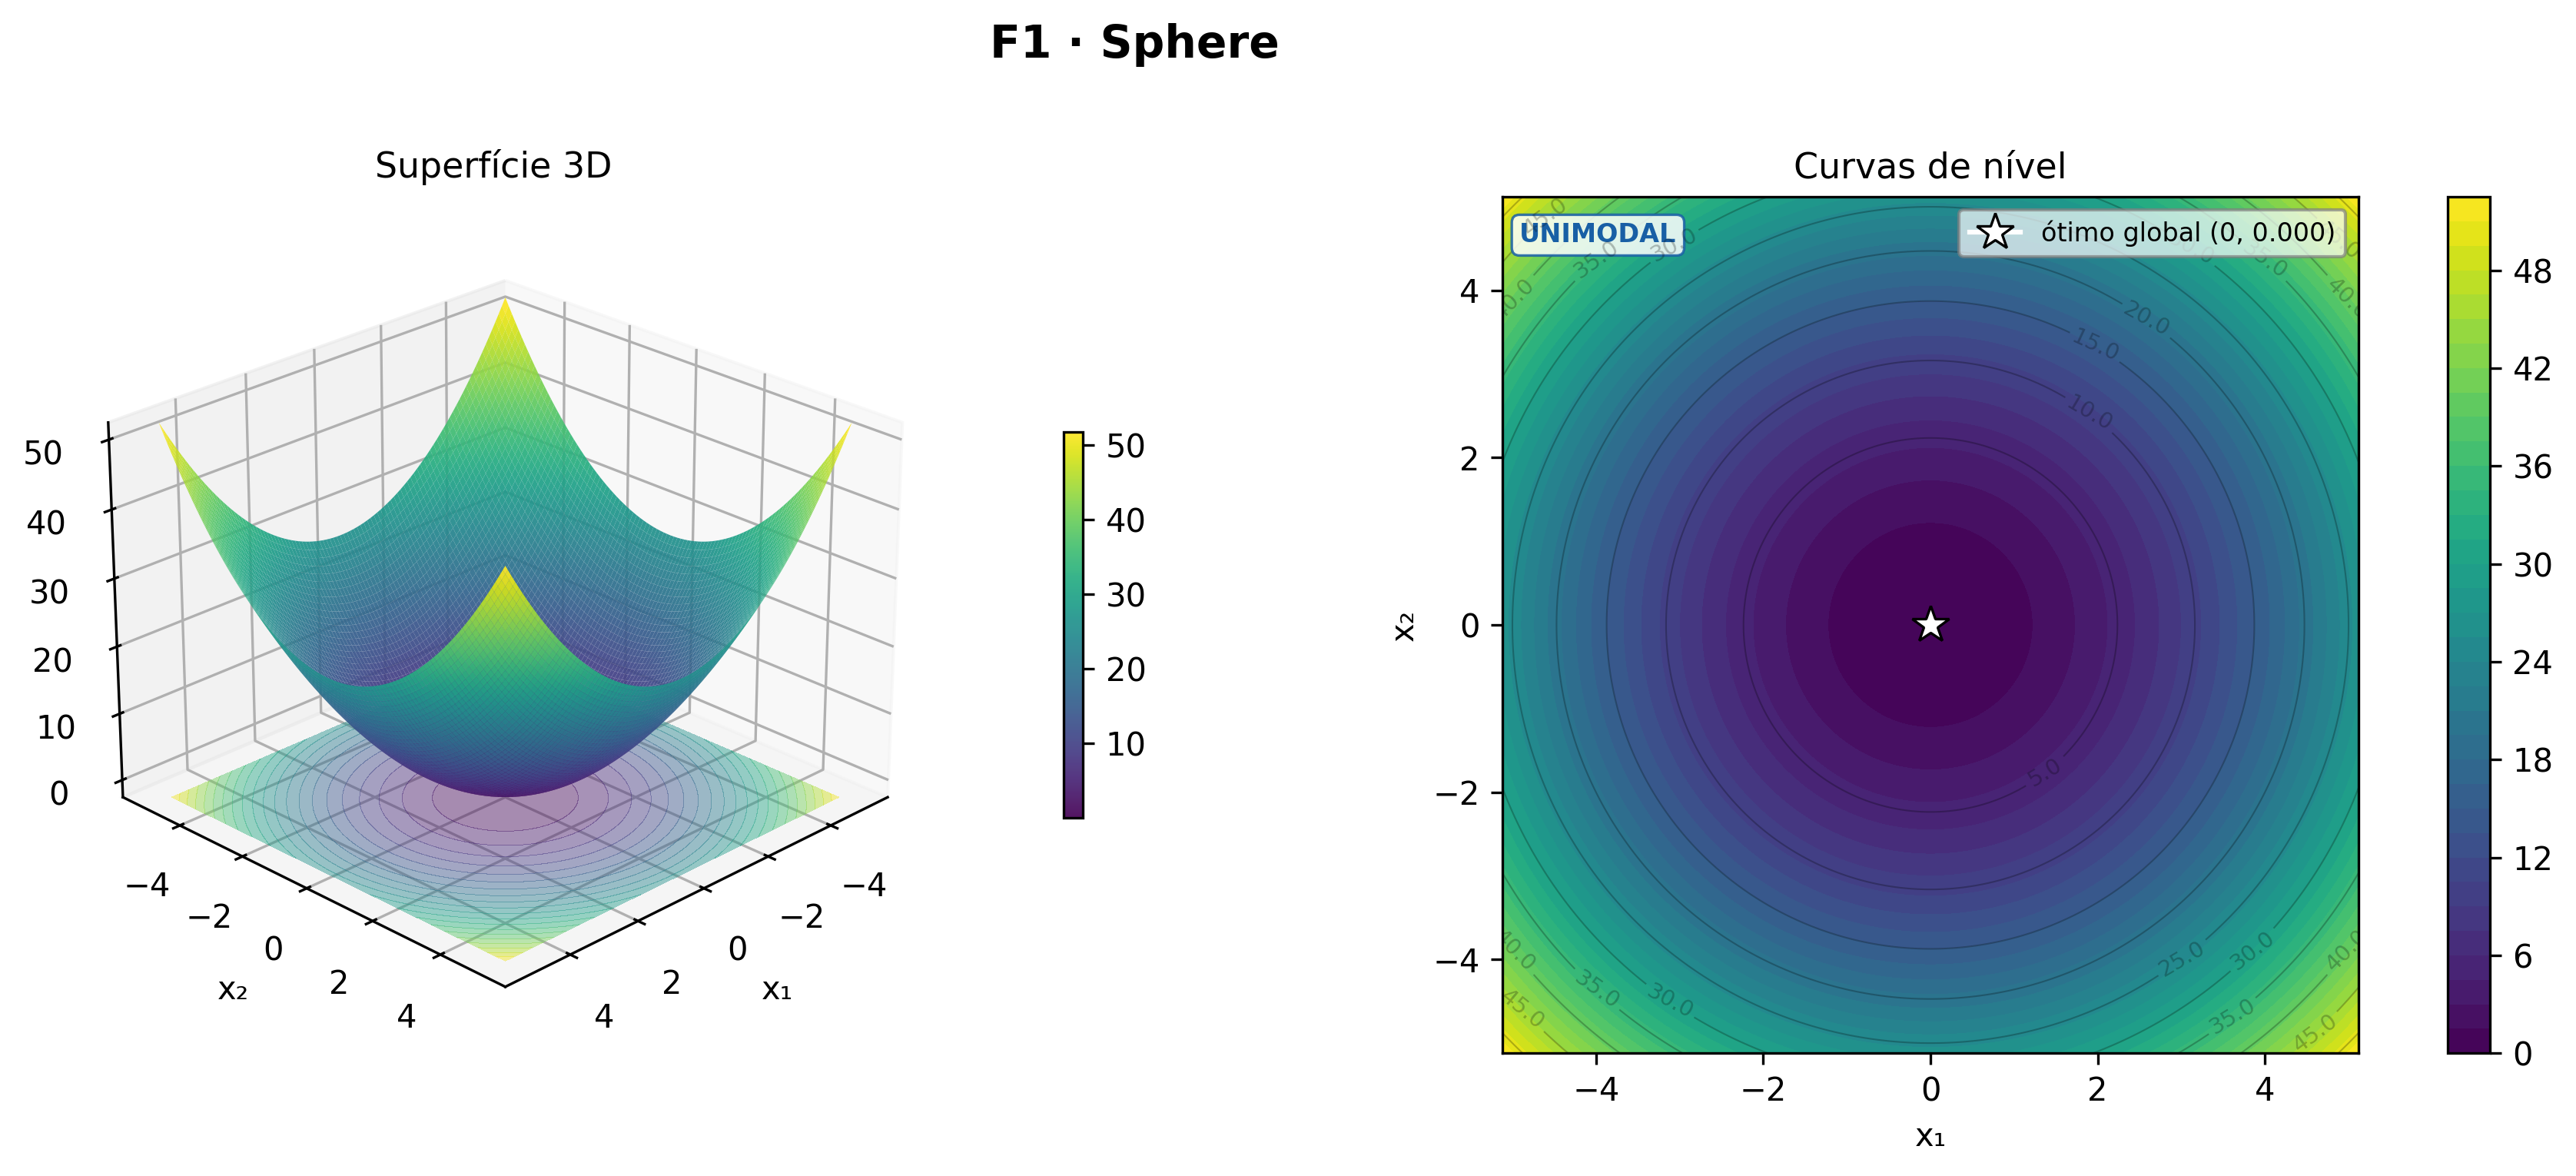
\includegraphics[width=0.75\textwidth]{figs/f1_sphere.png}
\caption{Superfície 3D e curvas de nível da função Sphere ($D=2$).}
\label{fig:sphere}
\end{figure}

\subsubsection{Rosenbrock}\leavevmode
$f(\mathbf{x}) = \sum_{i=1}^{D-1}\left[100(x_{i+1}-x_i^2)^2 +
(x_i-1)^2\right]$, domínio $[-5,\,10]^D$.
Não-separável; o ótimo global em $\mathbf{x}^*=(1,\ldots,1)$
localiza-se em um vale estreito e curvo que desafia a convergência
de metaheurísticas.

\begin{figure}[H]
\centering
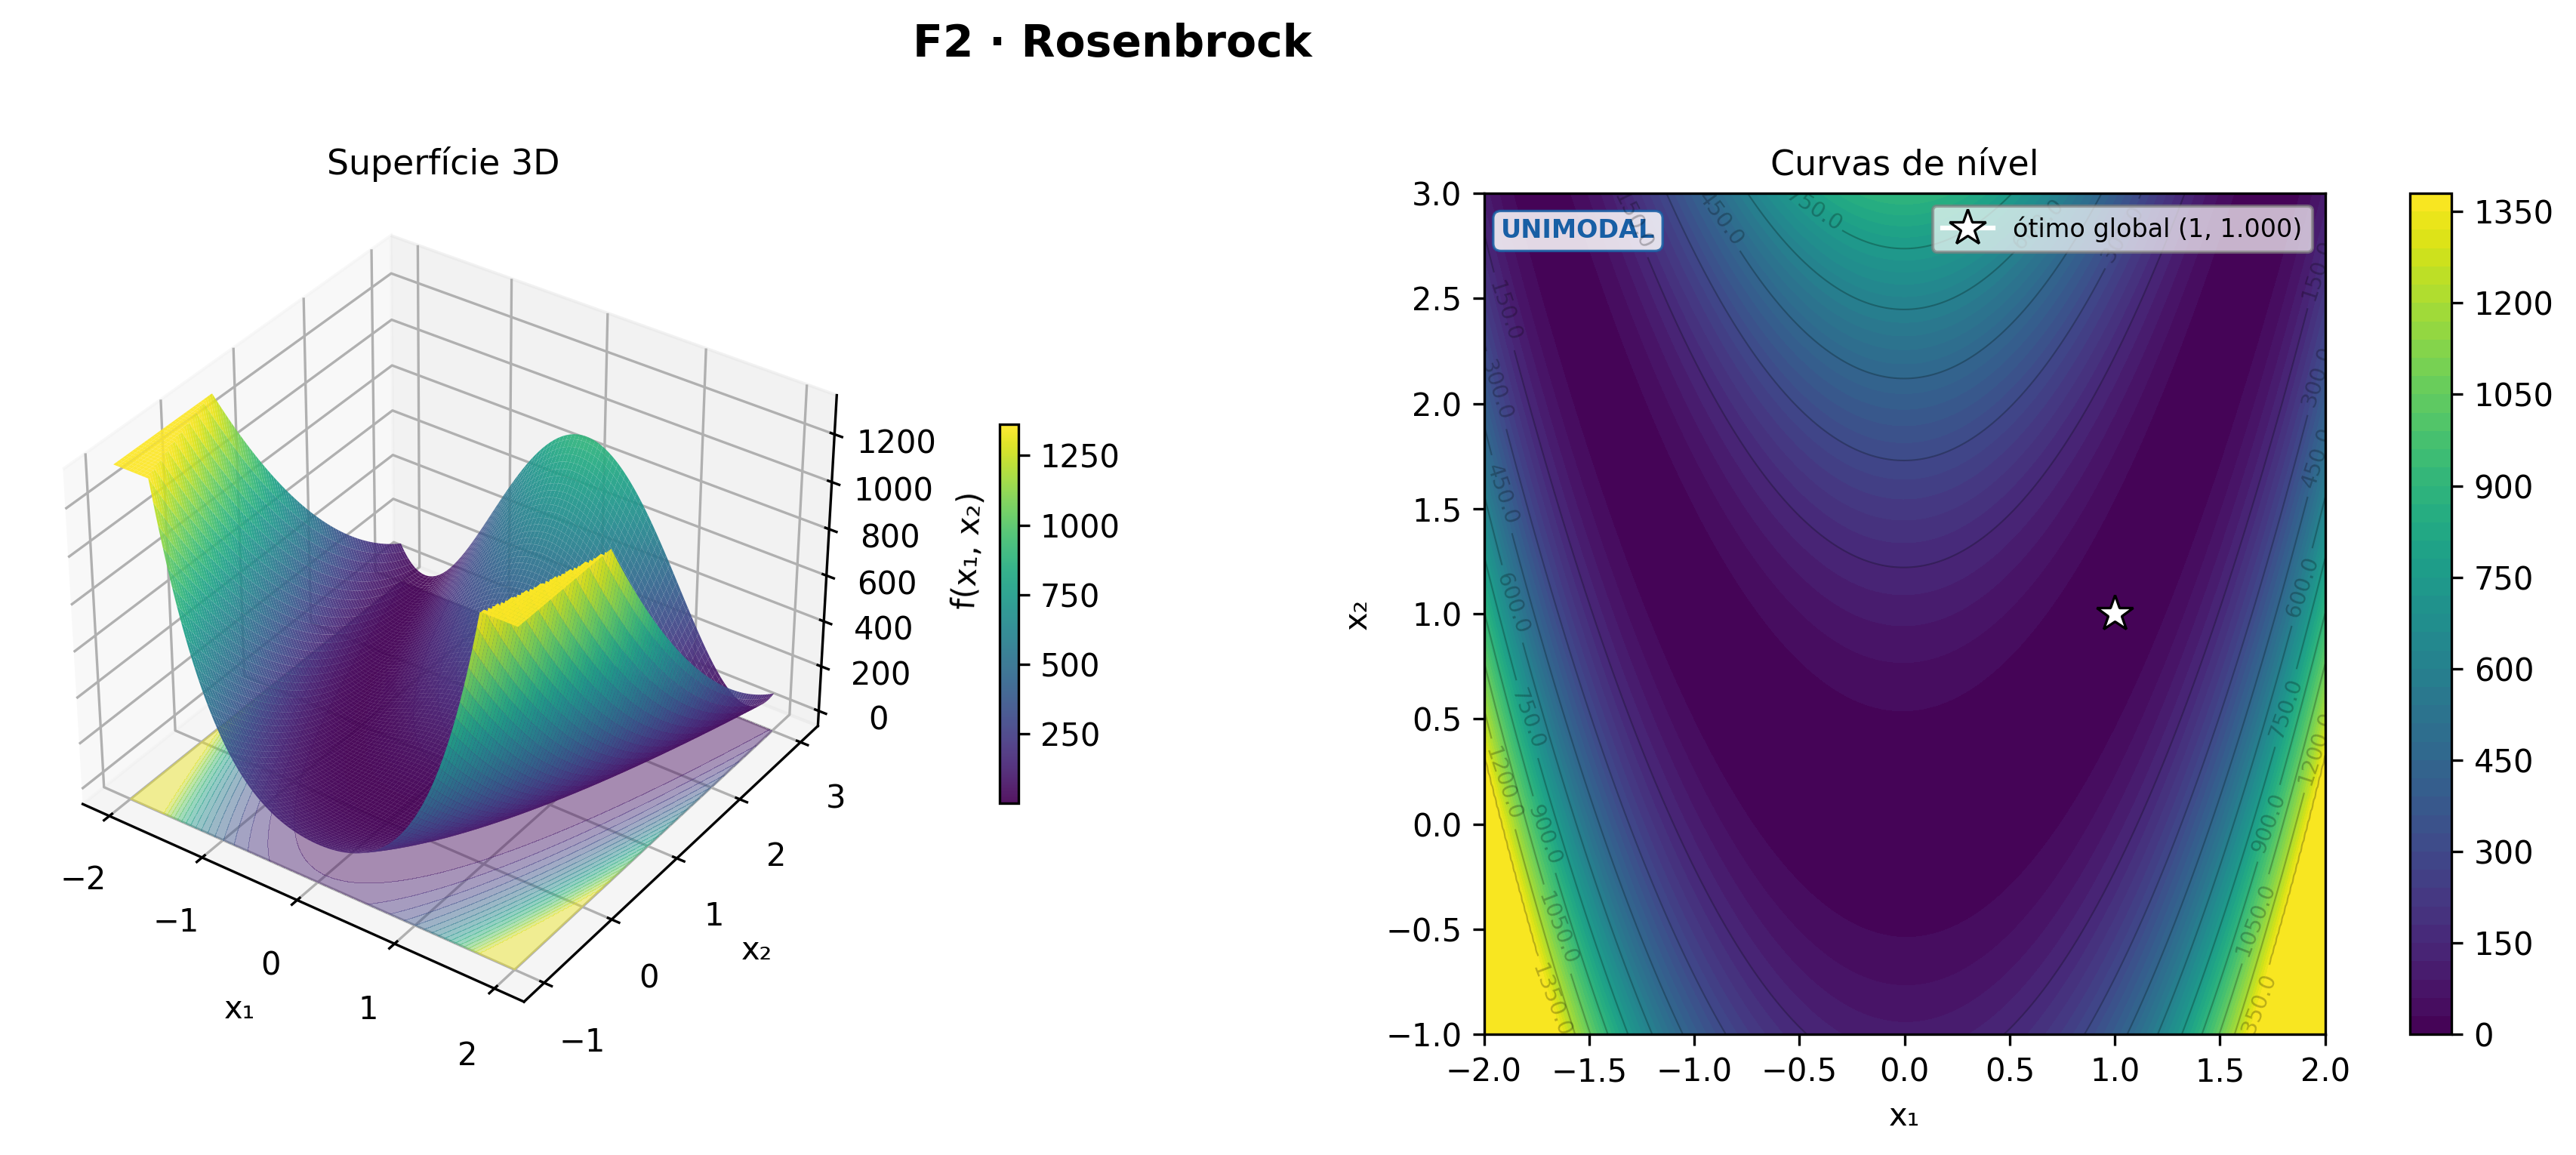
\includegraphics[width=0.75\textwidth]{figs/f2_·_rosenbrock.png}
\caption{Superfície 3D e curvas de nível da função Rosenbrock ($D=2$).}
\label{fig:rosenbrock}
\end{figure}

\subsubsection{Sum Squares}\leavevmode
$f(\mathbf{x}) = \sum_{i=1}^{D} i\,x_i^2$, domínio $[-10,\,10]^D$.
Separável com pesos crescentes por dimensão; introduz condicionamento
moderado sem redundância com outras funções unimodais do conjunto.

\begin{figure}[H]
\centering
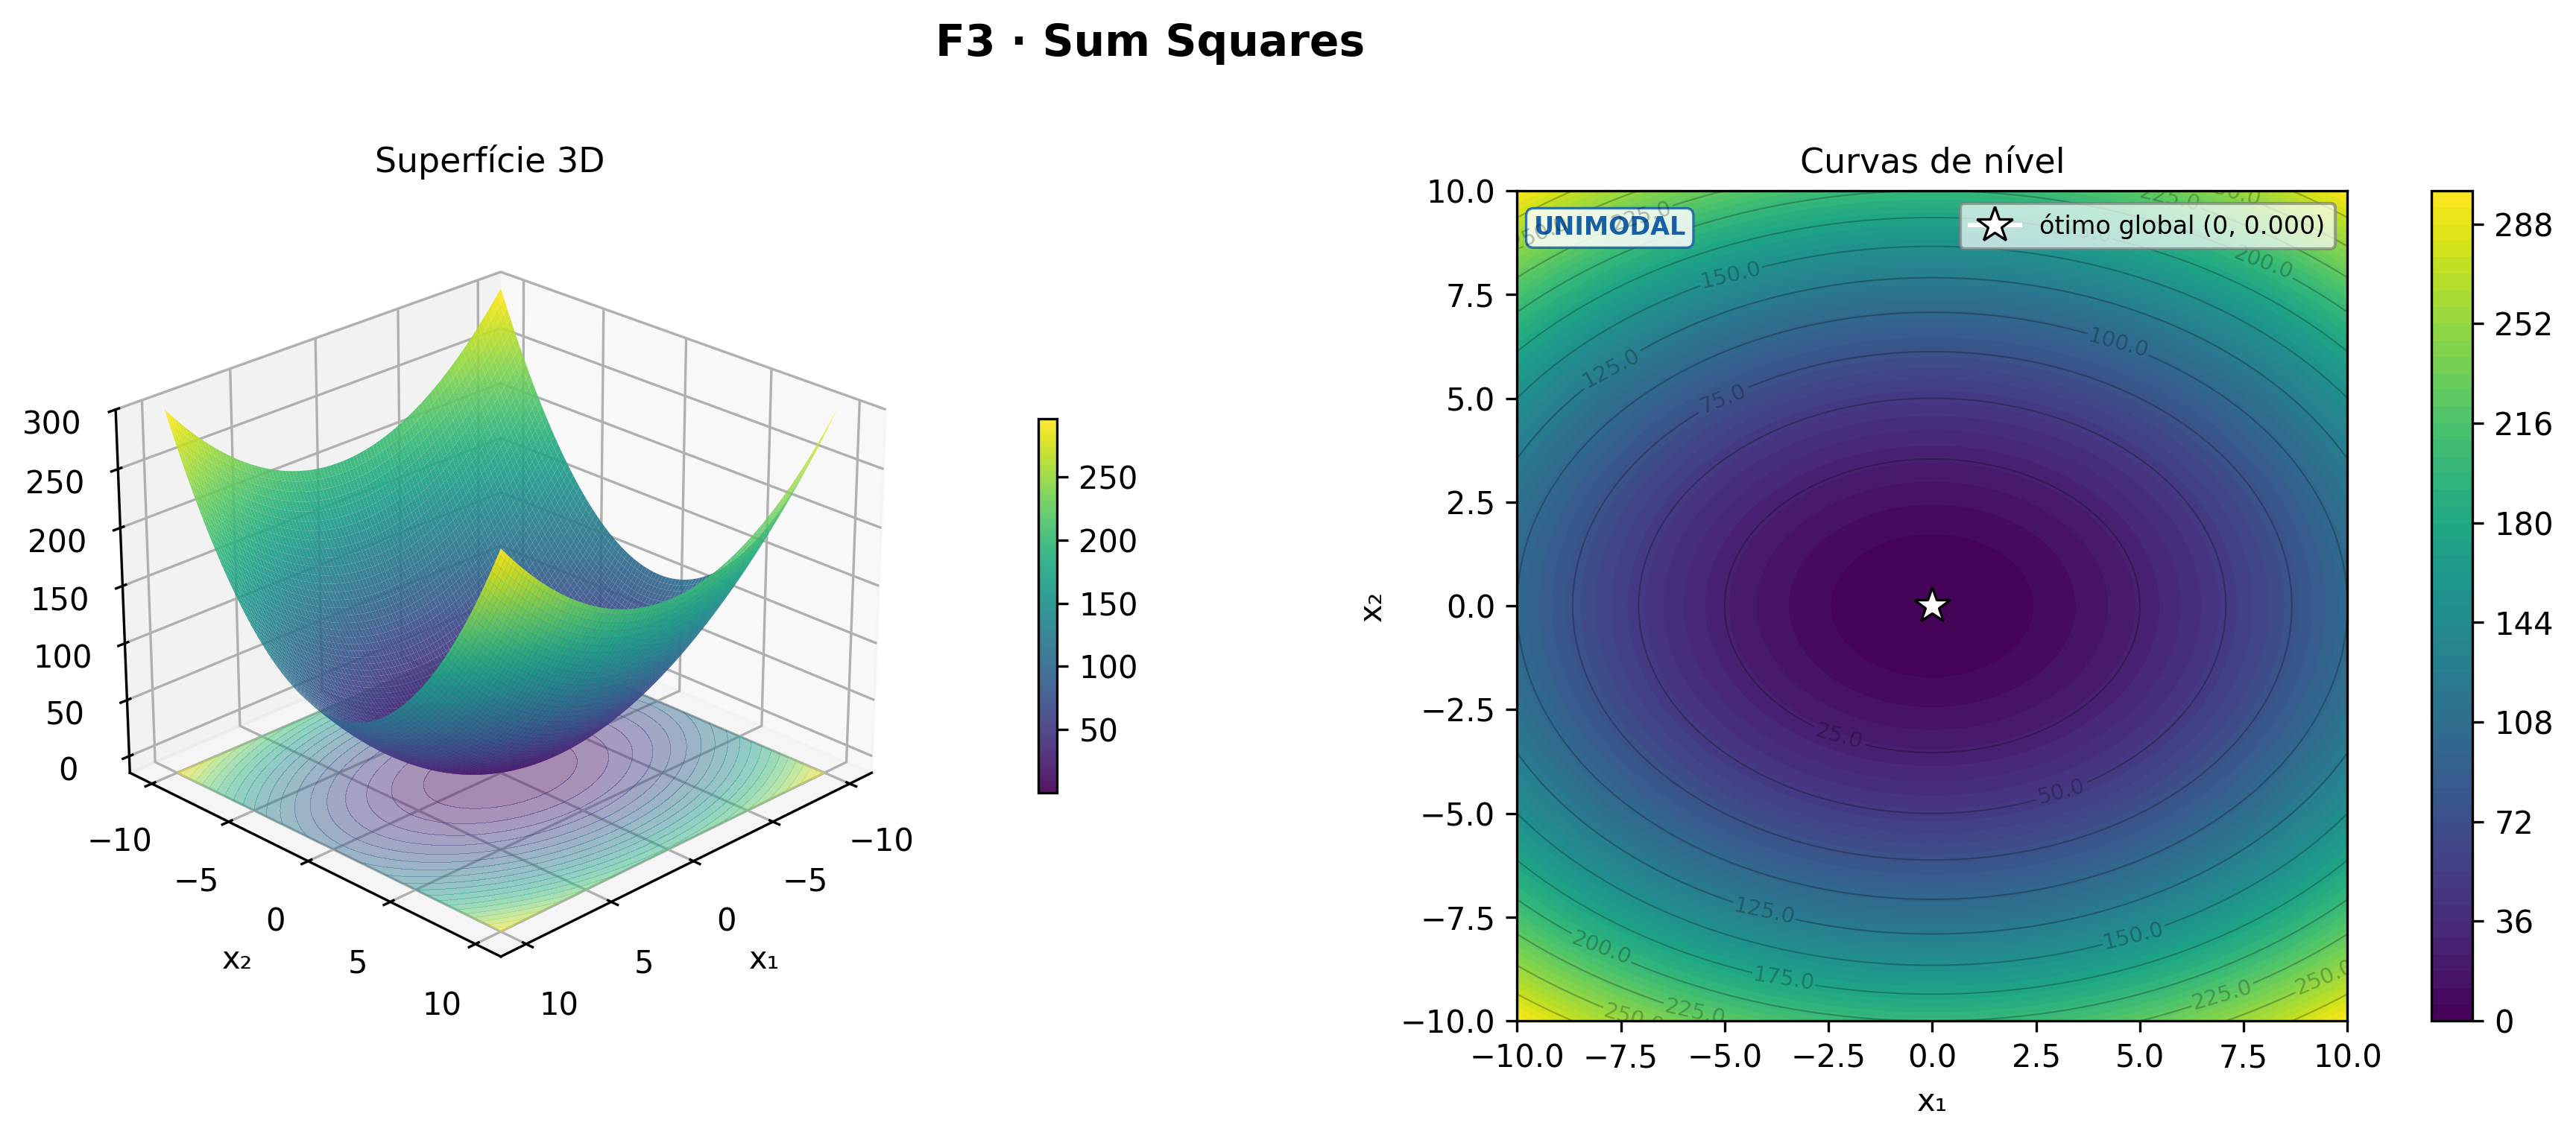
\includegraphics[width=0.75\textwidth]{figs/f3_·_sum_squares.png}
\caption{Superfície 3D e curvas de nível da função Sum Squares ($D=2$).}
\label{fig:sum_squares}
\end{figure}

\subsubsection{Dixon-Price}\leavevmode
$f(\mathbf{x}) = (x_1-1)^2 + \sum_{i=2}^{D}
i\,(2x_i^2 - x_{i-1})^2$, domínio $[-10,\,10]^D$.
Não-separável com ótimo analítico
$x_i^* = 2^{-(2^i-2)/2^i}$; útil para validar a convergência
em estrutura recursiva de vale diagonal.

\begin{figure}[H]
\centering
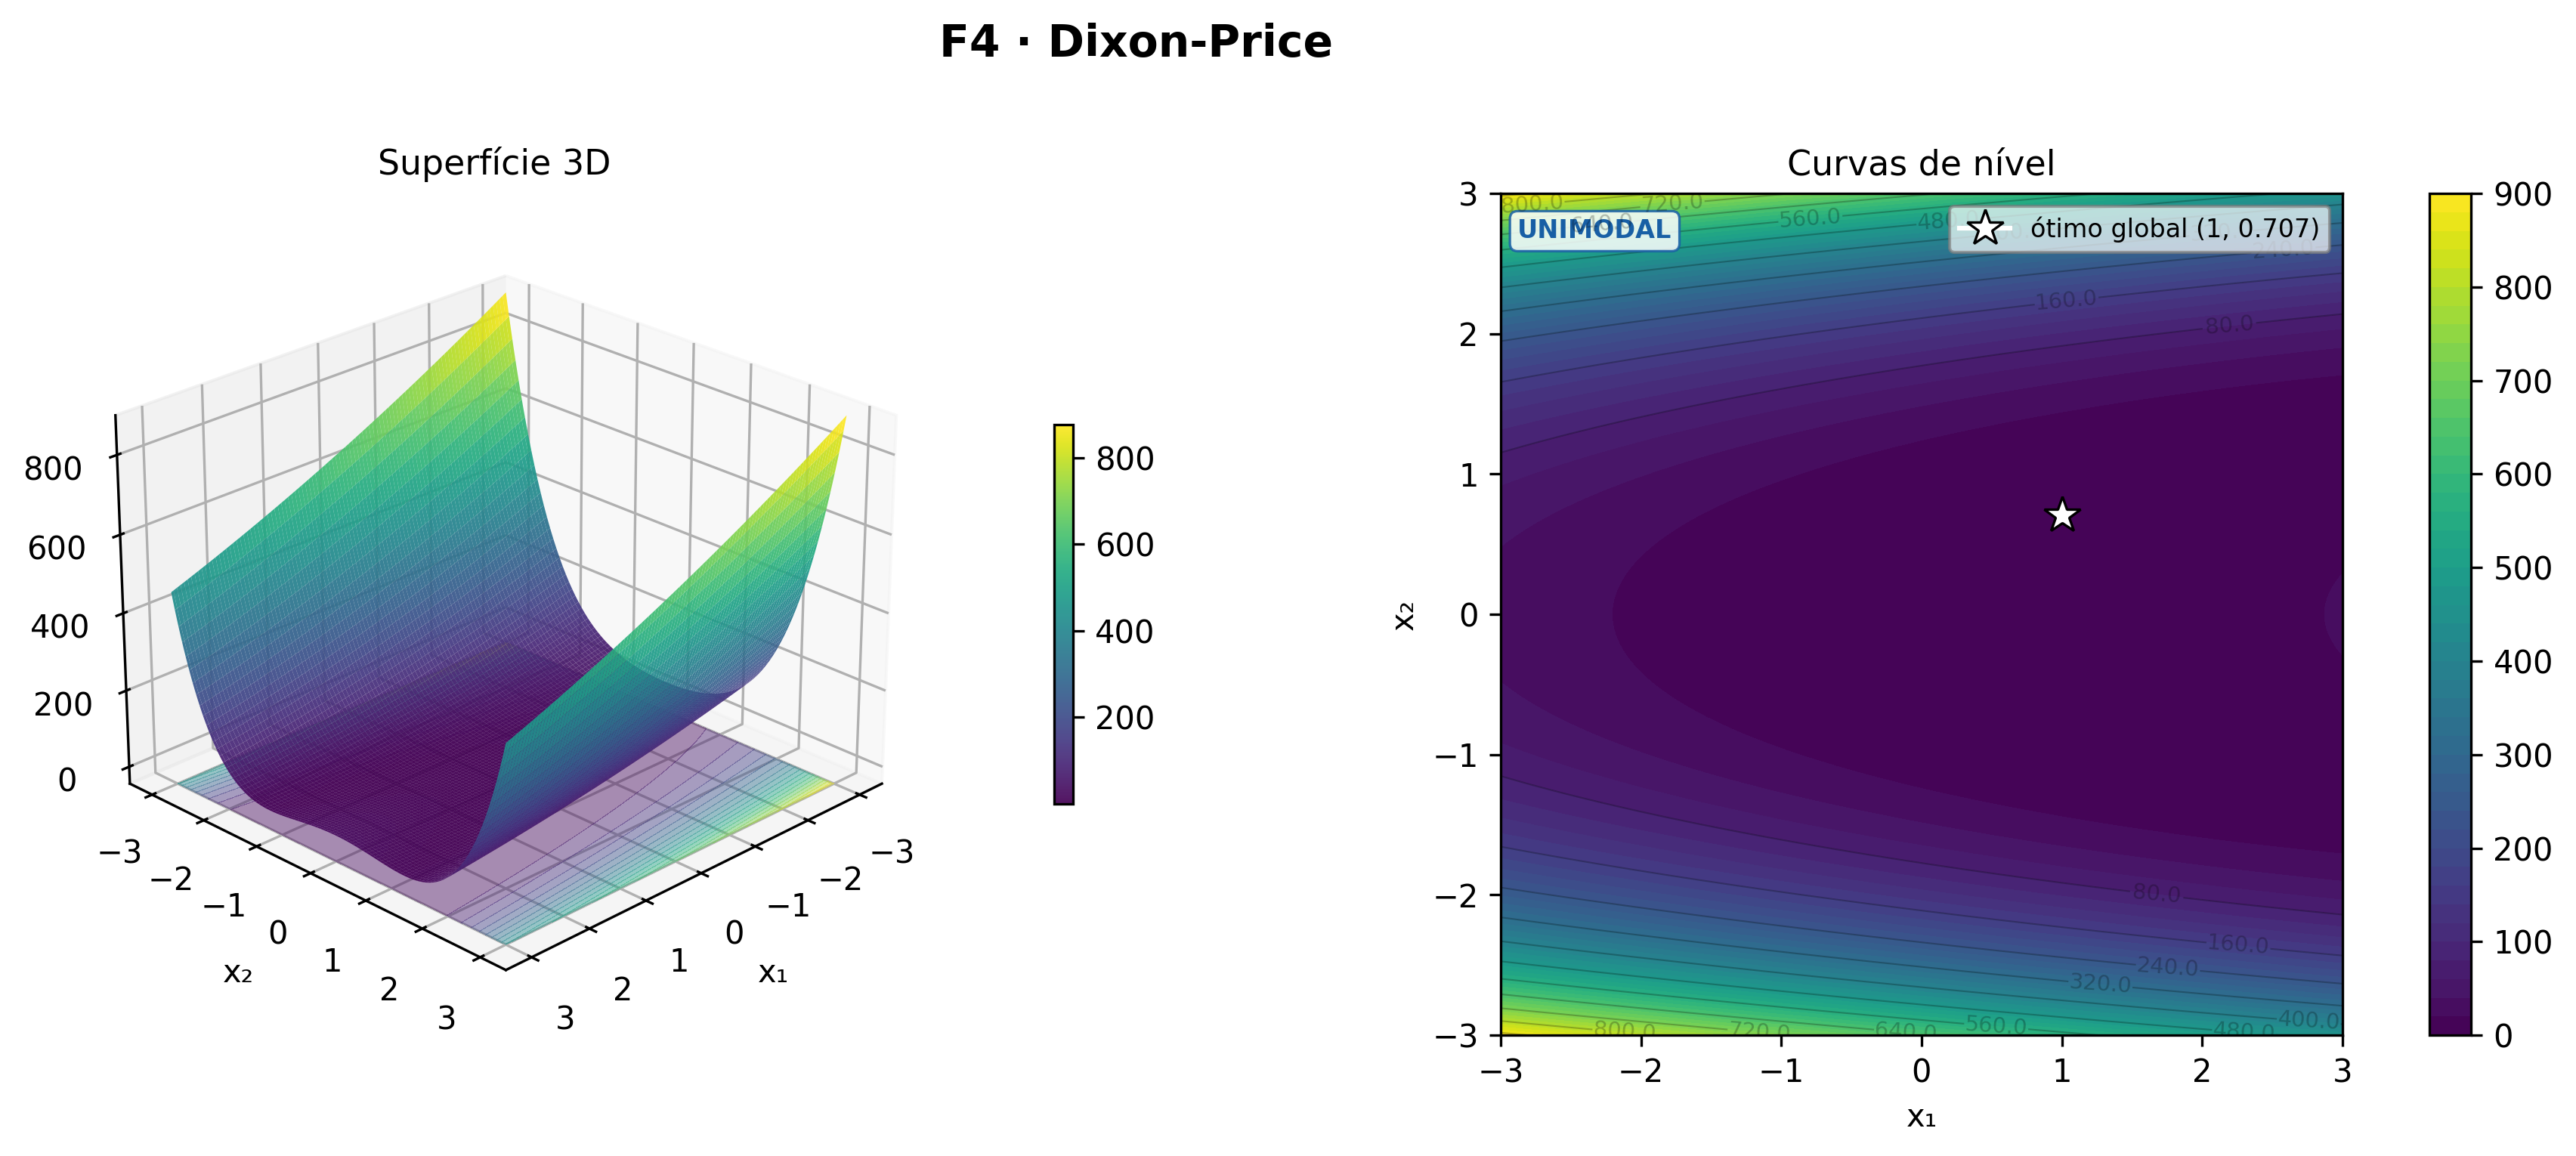
\includegraphics[width=0.75\textwidth]{figs/f4_·_dixon-price.png}
\caption{Superfície 3D e curvas de nível da função Dixon-Price ($D=2$).}
\label{fig:dixon_price}
\end{figure}

\subsubsection{Zakharov}\leavevmode
$f(\mathbf{x}) = \sum_{i=1}^{D}x_i^2 +
\left(\sum_{i=1}^{D}0{,}5\,i\,x_i\right)^2 +
\left(\sum_{i=1}^{D}0{,}5\,i\,x_i\right)^4$,
domínio $[-5,\,10]^D$.
Unimodal não-separável com crescimento polinomial misto; avalia a
capacidade de coordenação entre dimensões.

\begin{figure}[H]
\centering
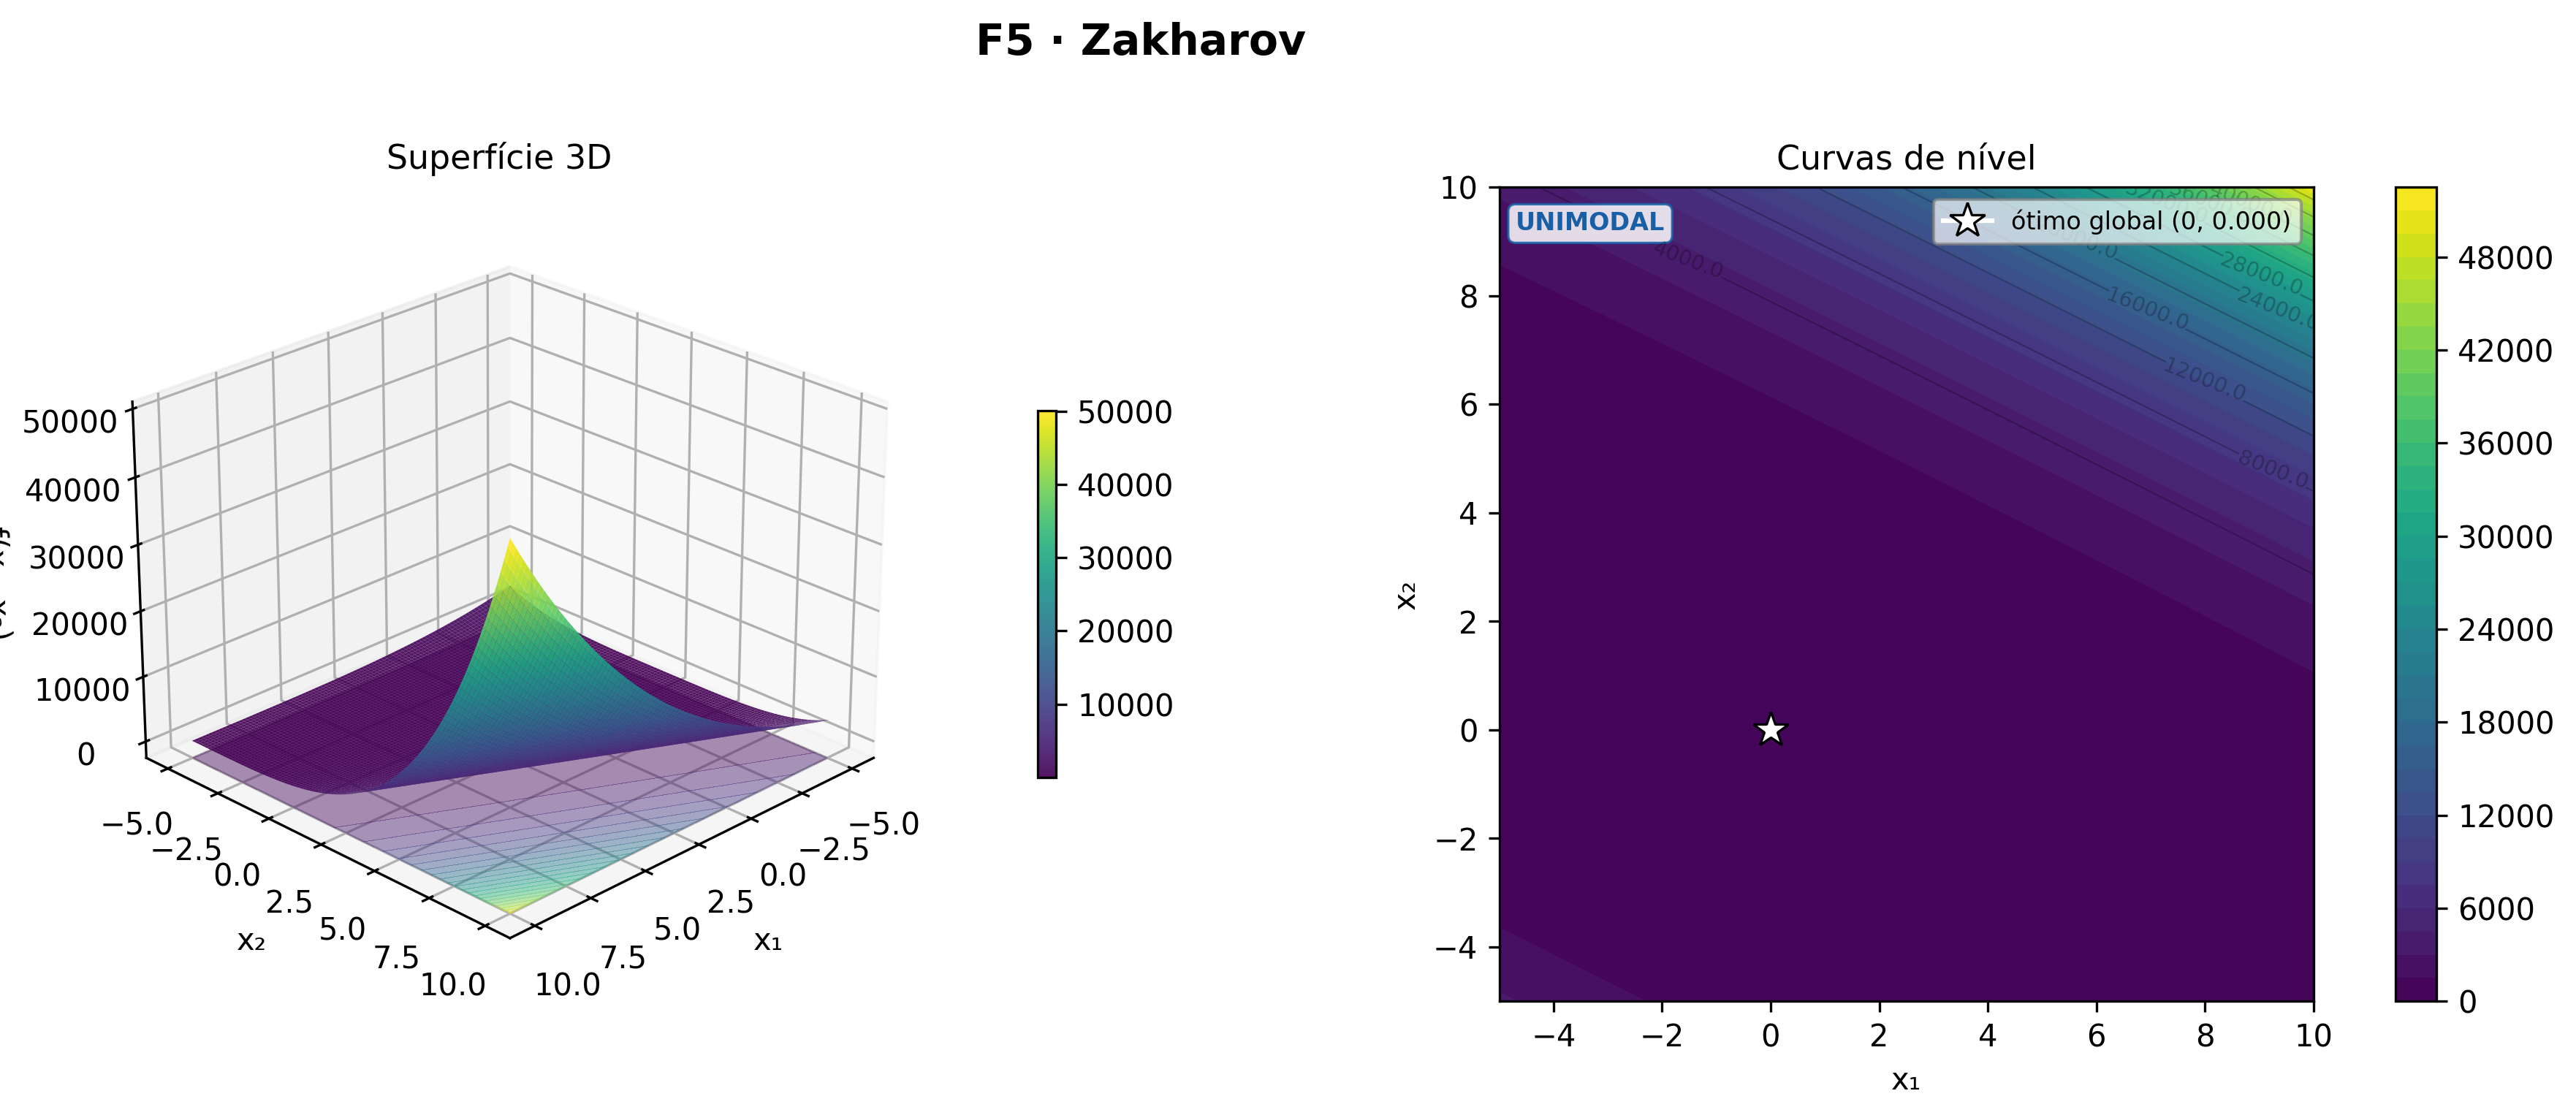
\includegraphics[width=0.75\textwidth]{figs/f5_·_zakharov.png}
\caption{Superfície 3D e curvas de nível da função Zakharov ($D=2$).}
\label{fig:zakharov}
\end{figure}

\subsection{Fun\c{c}\~{o}es Multimodais}

\subsubsection{Rastrigin}\leavevmode
$f(\mathbf{x}) = 10D + \sum_{i=1}^{D}\left[x_i^2 -
10\cos(2\pi x_i)\right]$, domínio $[-5{,}12,\,5{,}12]^D$.
Separável com grade densa de ótimos locais; referência clássica para
avaliar diversidade e capacidade de escape de mínimos locais.

\begin{figure}[H]
\centering
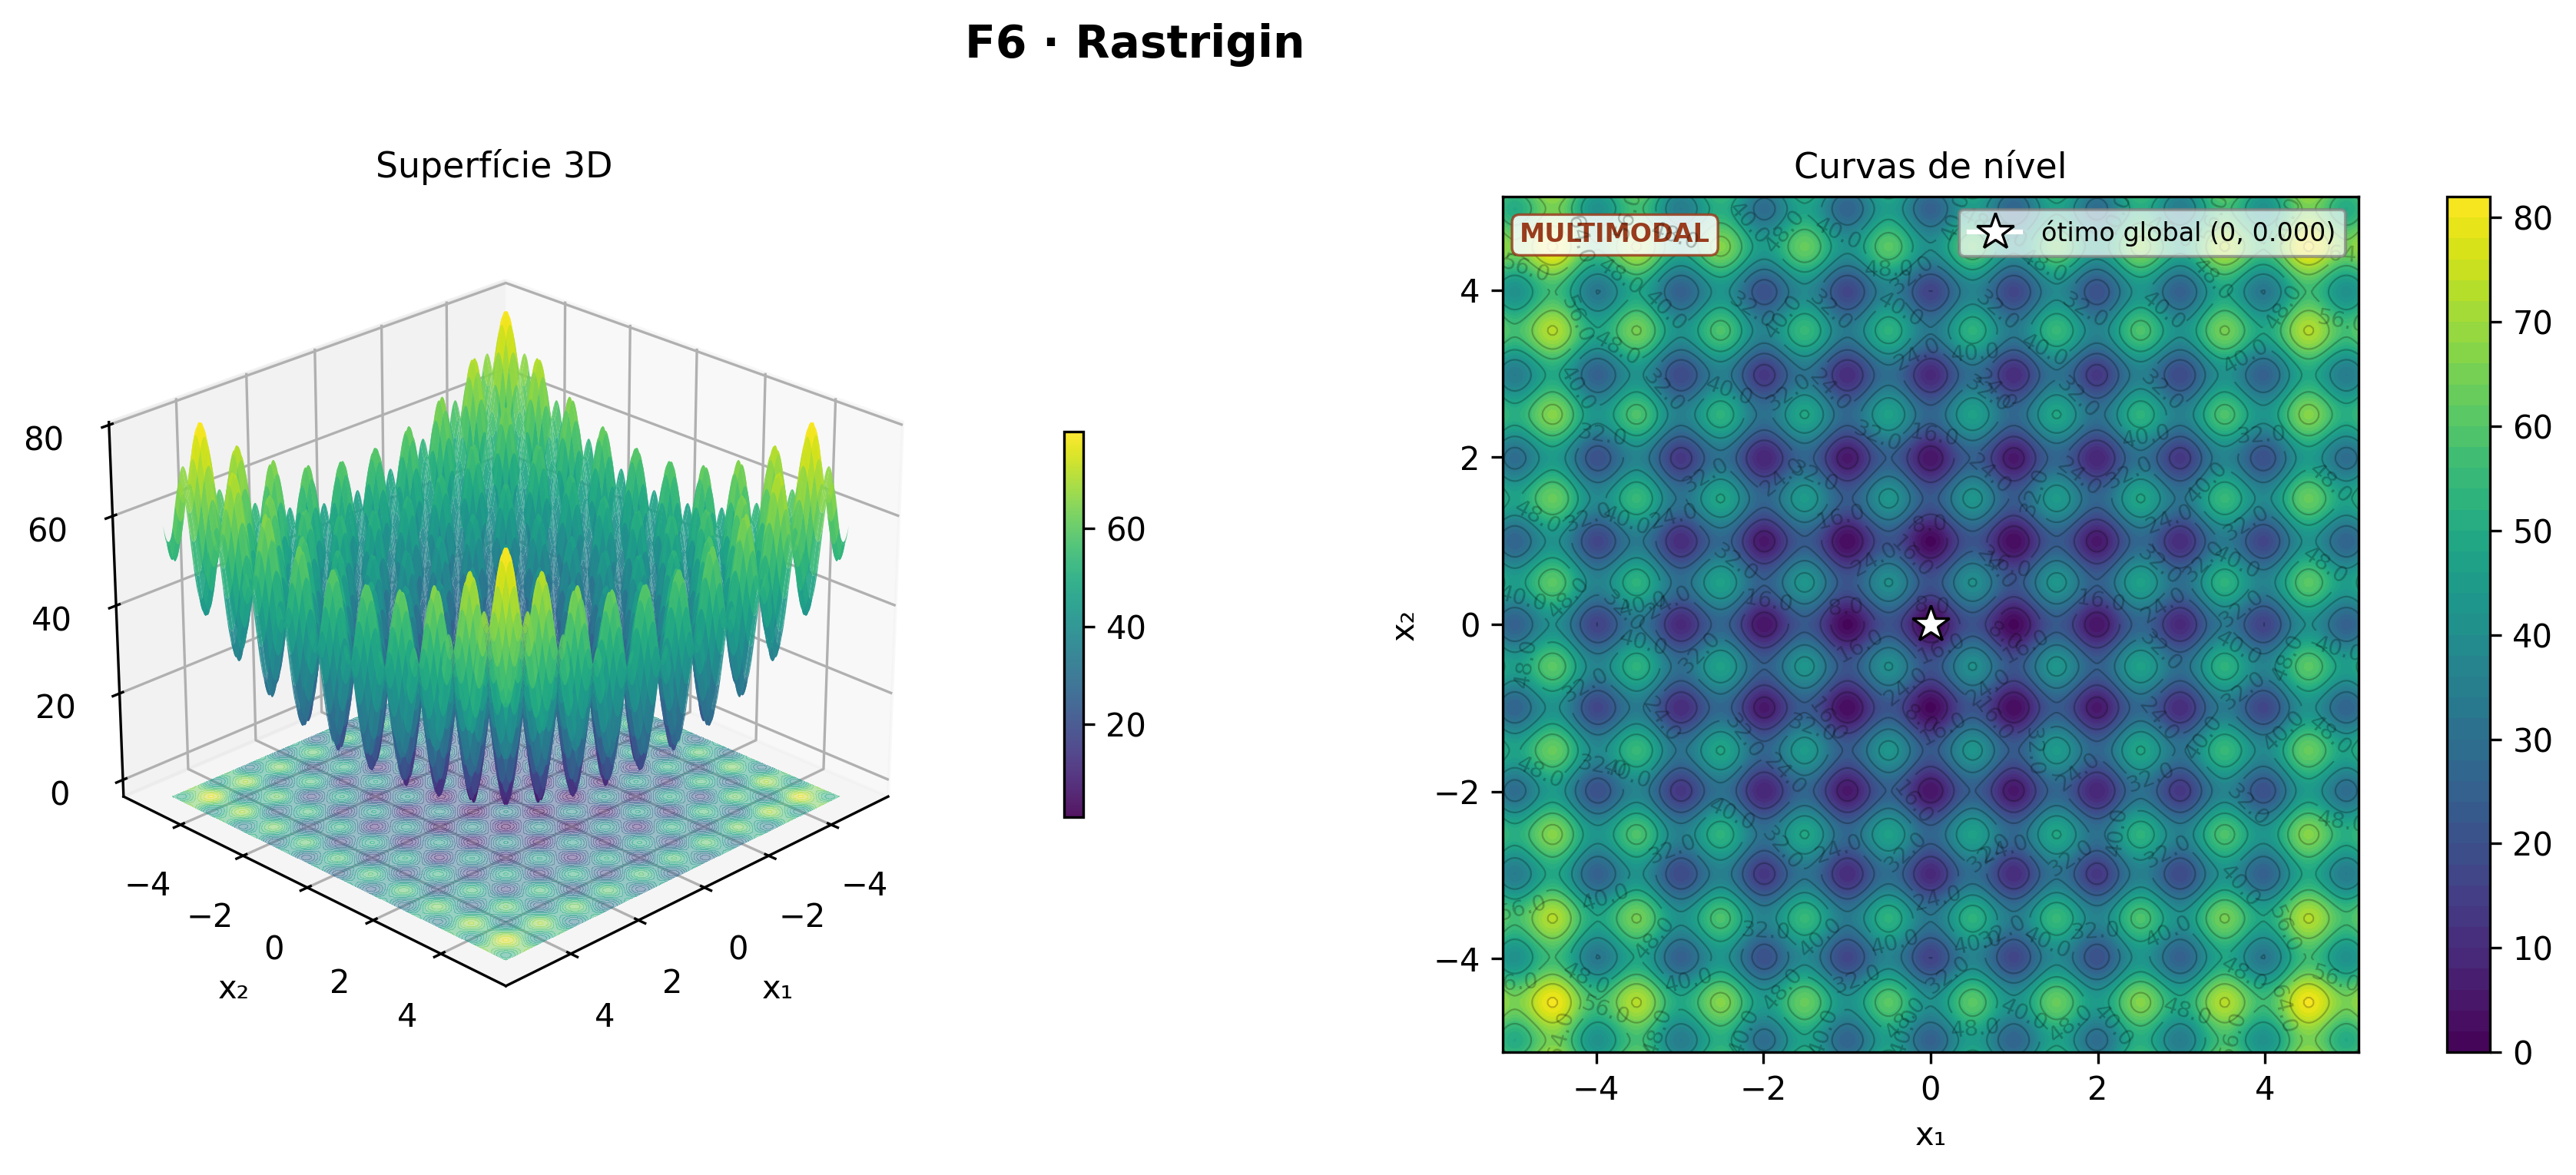
\includegraphics[width=0.75\textwidth]{figs/f6_·_rastrigin.png}
\caption{Superfície 3D e curvas de nível da função Rastrigin ($D=2$).}
\label{fig:rastrigin}
\end{figure}

\subsubsection{Ackley}\leavevmode
$f(\mathbf{x}) = -20\exp\!\left(-0{,}2\sqrt{\frac{1}{D}
\sum x_i^2}\right) - \exp\!\left(\frac{1}{D}\sum\cos 2\pi x_i\right)
+ 20 + e$, domínio $[-32{,}768,\,32{,}768]^D$.
Apresenta um platô amplo com um pico central estreito, criando
armadilha para algoritmos gulosos.

\begin{figure}[H]
\centering
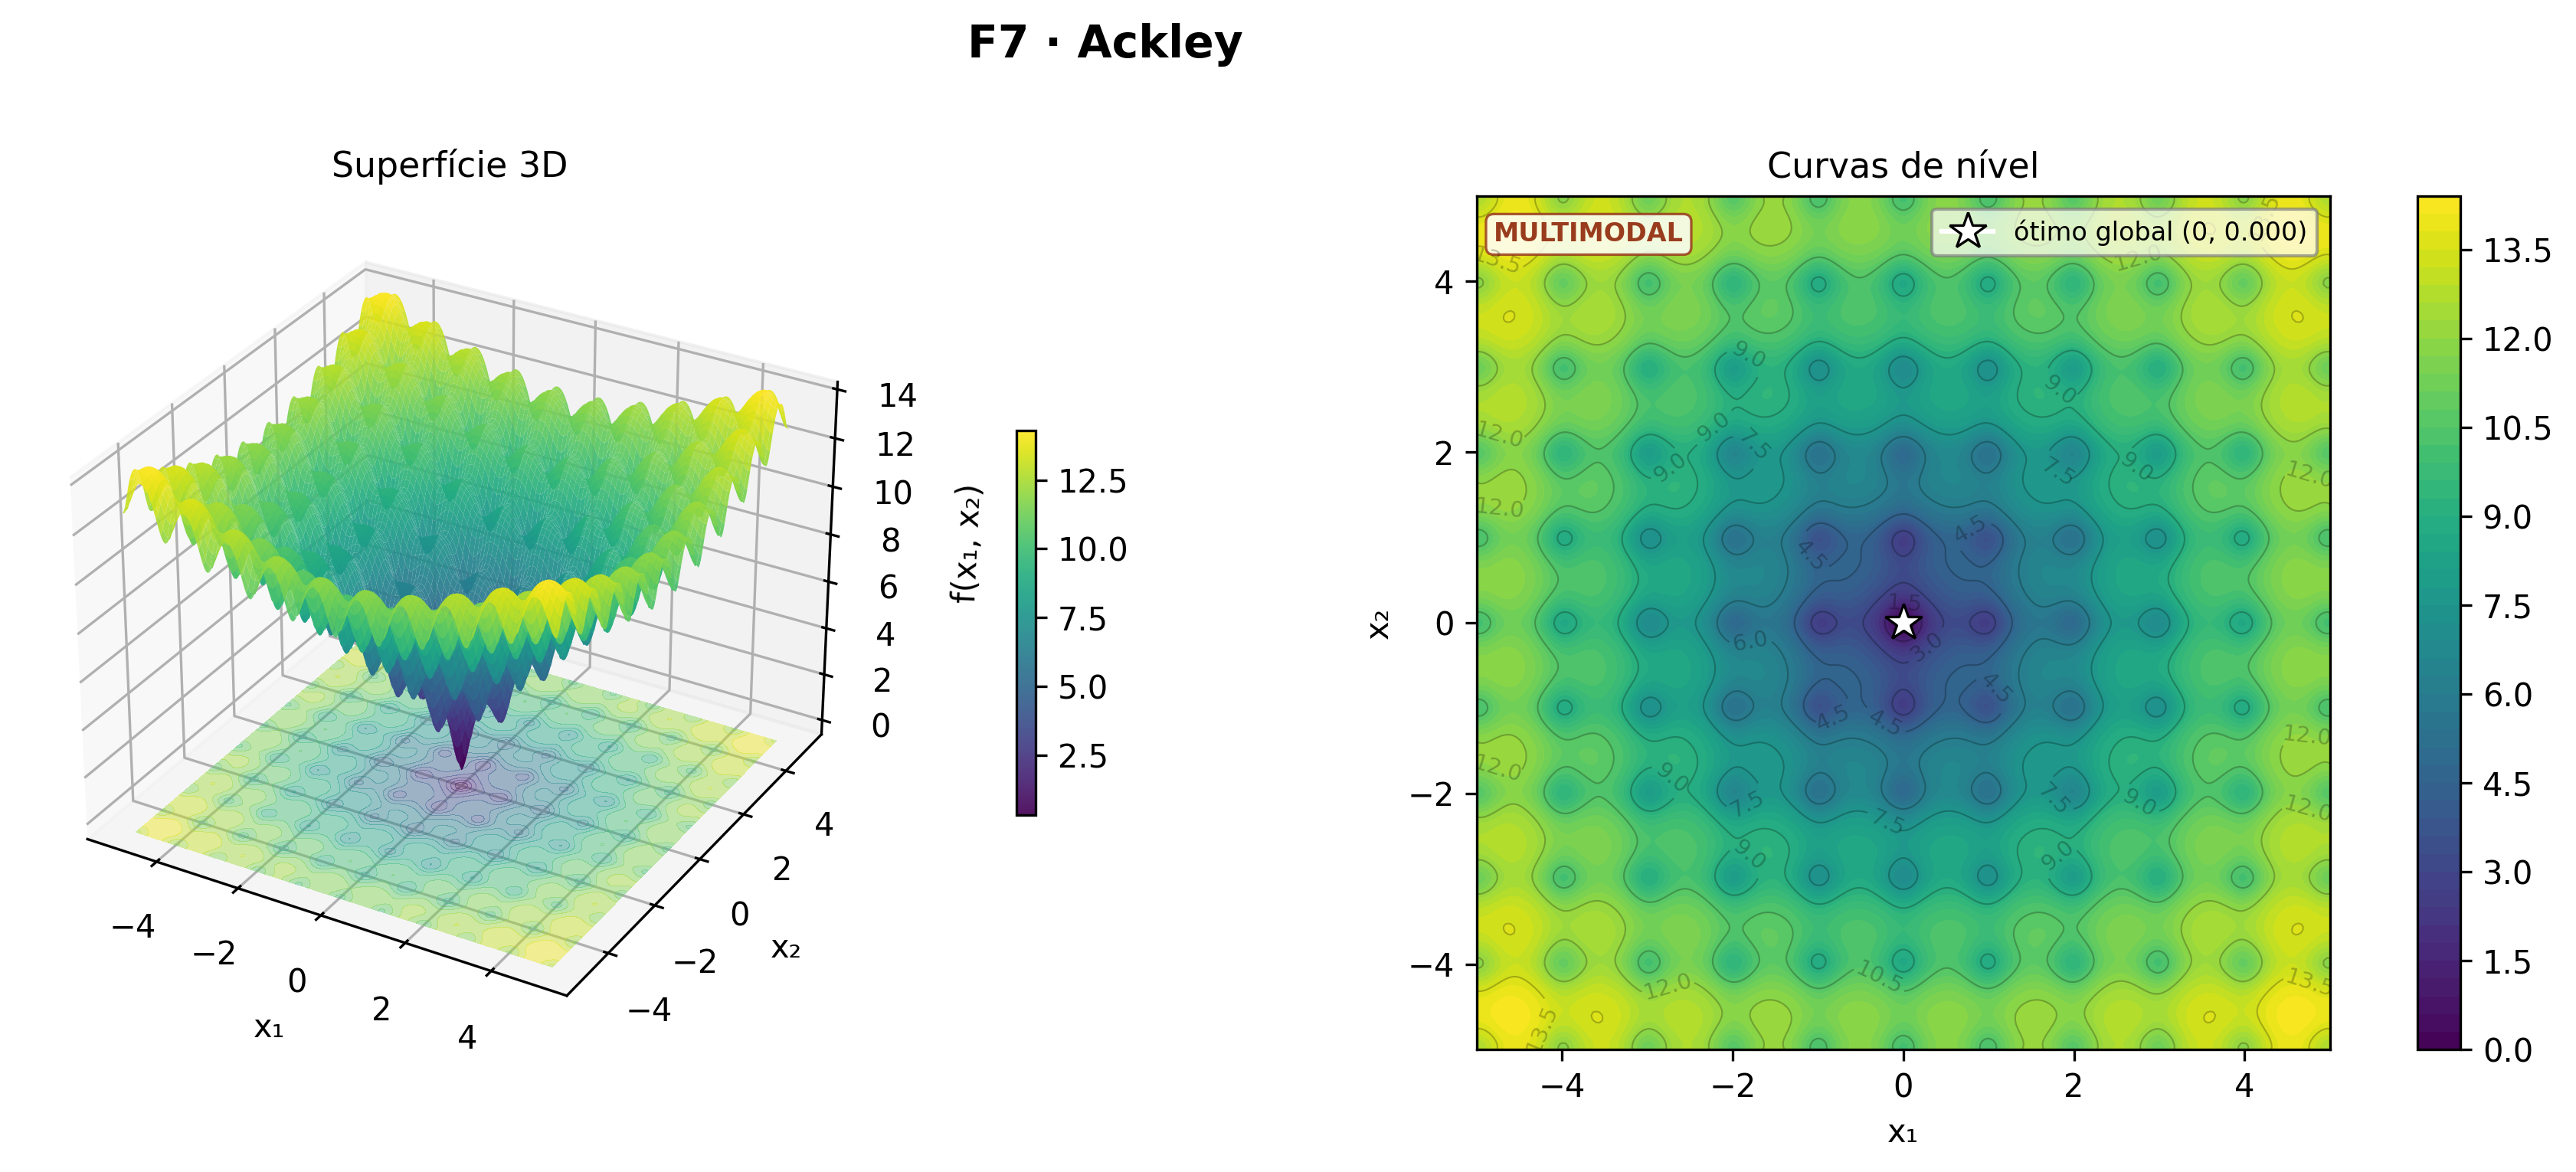
\includegraphics[width=0.75\textwidth]{figs/f7_·_ackley.png}
\caption{Superfície 3D e curvas de nível da função Ackley ($D=2$).}
\label{fig:ackley}
\end{figure}

\subsubsection{Griewank}\leavevmode
$f(\mathbf{x}) = \frac{1}{4000}\sum x_i^2 -
\prod_{i=1}^{D}\cos\!\left(\frac{x_i}{\sqrt{i}}\right) + 1$,
domínio $[-600,\,600]^D$.
Multimodal não-separável; a dificuldade aumenta com $D$ devido ao
produto de cossenos.

\begin{figure}[H]
\centering
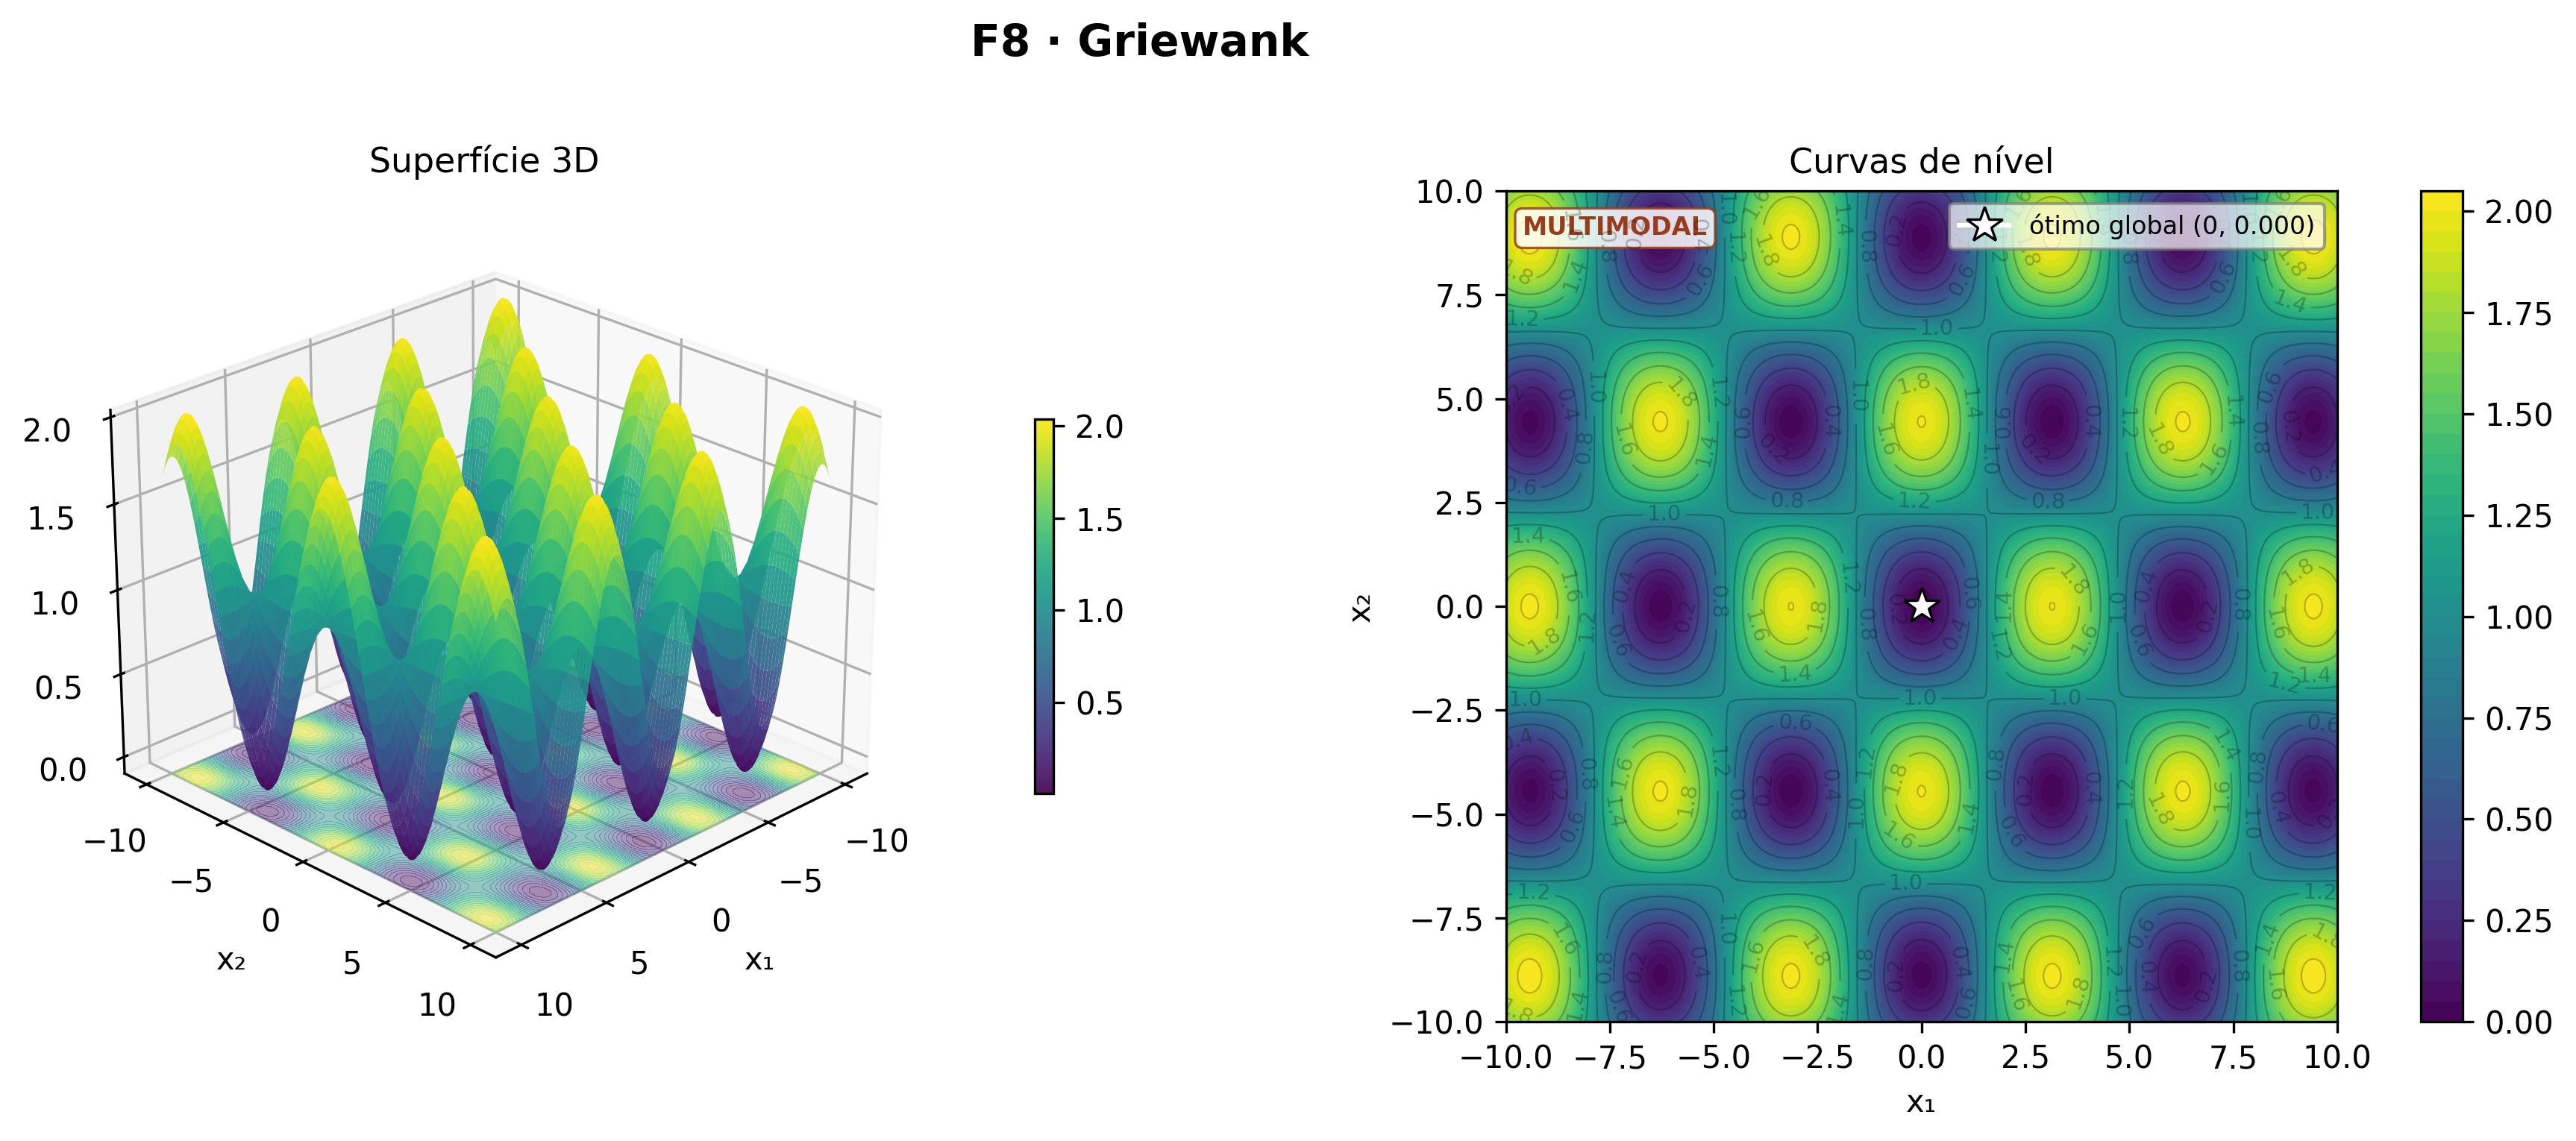
\includegraphics[width=0.75\textwidth]{figs/f8_·_griewank.png}
\caption{Superfície 3D e curvas de nível da função Griewank ($D=2$).}
\label{fig:griewank}
\end{figure}

\subsubsection{Schwefel 2.26}\leavevmode
$f(\mathbf{x}) = 418{,}9829\,D -
\sum_{i=1}^{D} x_i \sin\!\left(\sqrt{|x_i|}\right)$,
domínio $[-500,\,500]^D$.
Separável e deceptiva: o ótimo global em $x_i^* \approx 420{,}97$
está na periferia do espaço de busca, distante do centro onde os
algoritmos tendem a inicializar.

\begin{figure}[H]
\centering
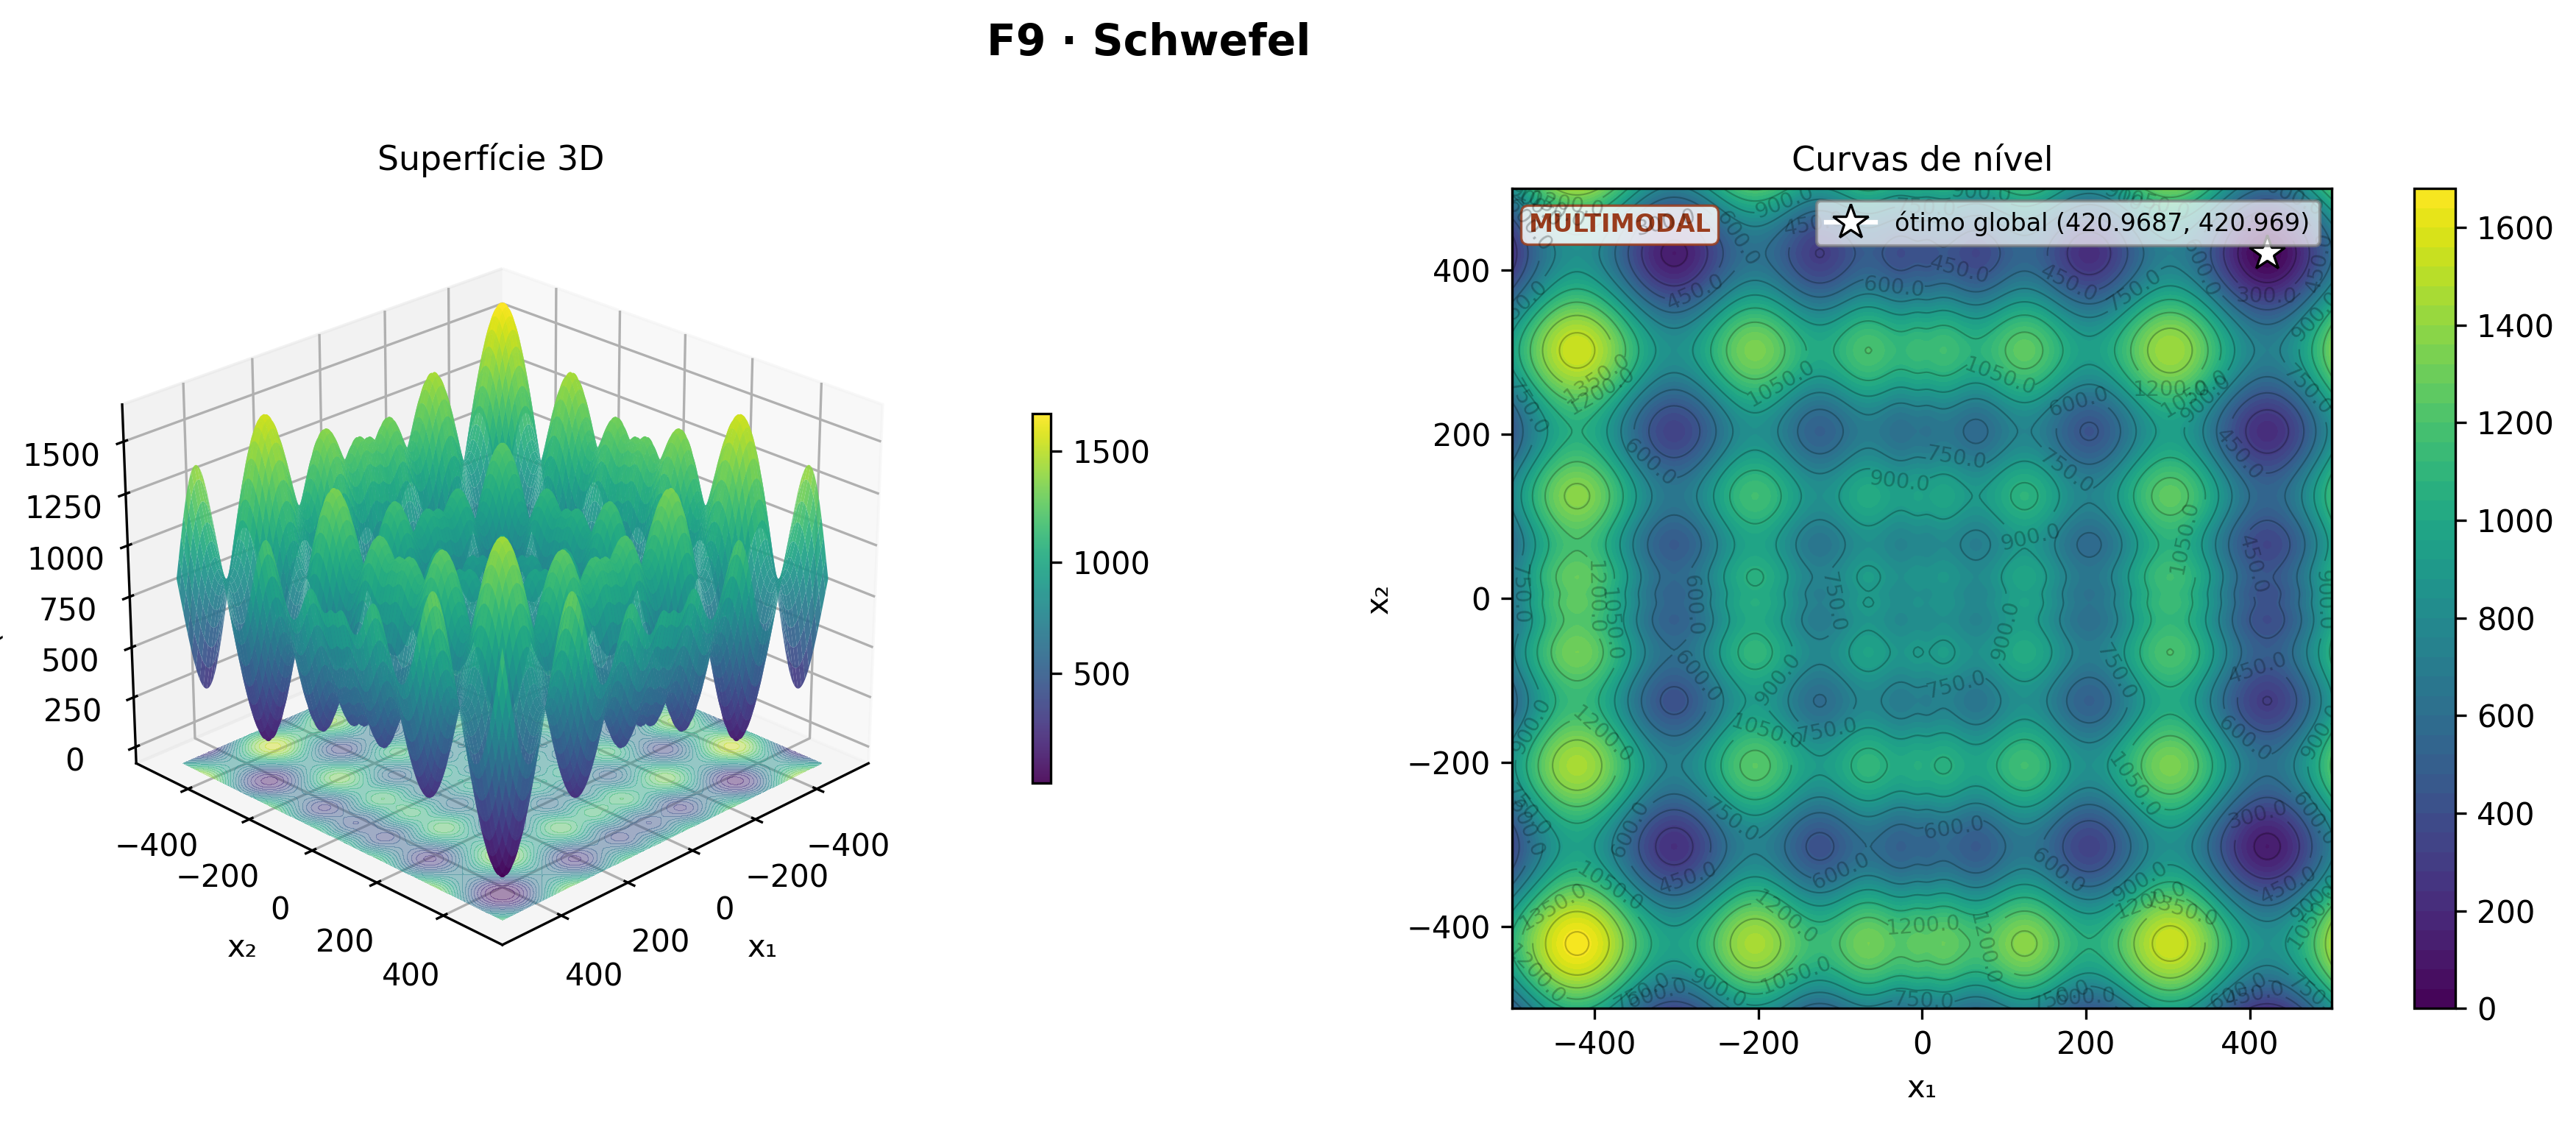
\includegraphics[width=0.75\textwidth]{figs/f9_·_schwefel.png}
\caption{Superfície 3D e curvas de nível da função Schwefel 2.26 ($D=2$).}
\label{fig:schwefel}
\end{figure}

\subsubsection{Lévy}\leavevmode
$f(\mathbf{x}) = \sin^2(\pi w_1) +
\sum_{i=1}^{D-1}(w_i-1)^2\left[1+10\sin^2(\pi w_{i+1})\right]
+ (w_D-1)^2\left[1+\sin^2(2\pi w_D)\right]$,
onde $w_i = 1 + (x_i-1)/4$, domínio $[-10,\,10]^D$.
Multimodal não-separável com ótimo único de localização não-trivial.

\begin{figure}[H]
\centering
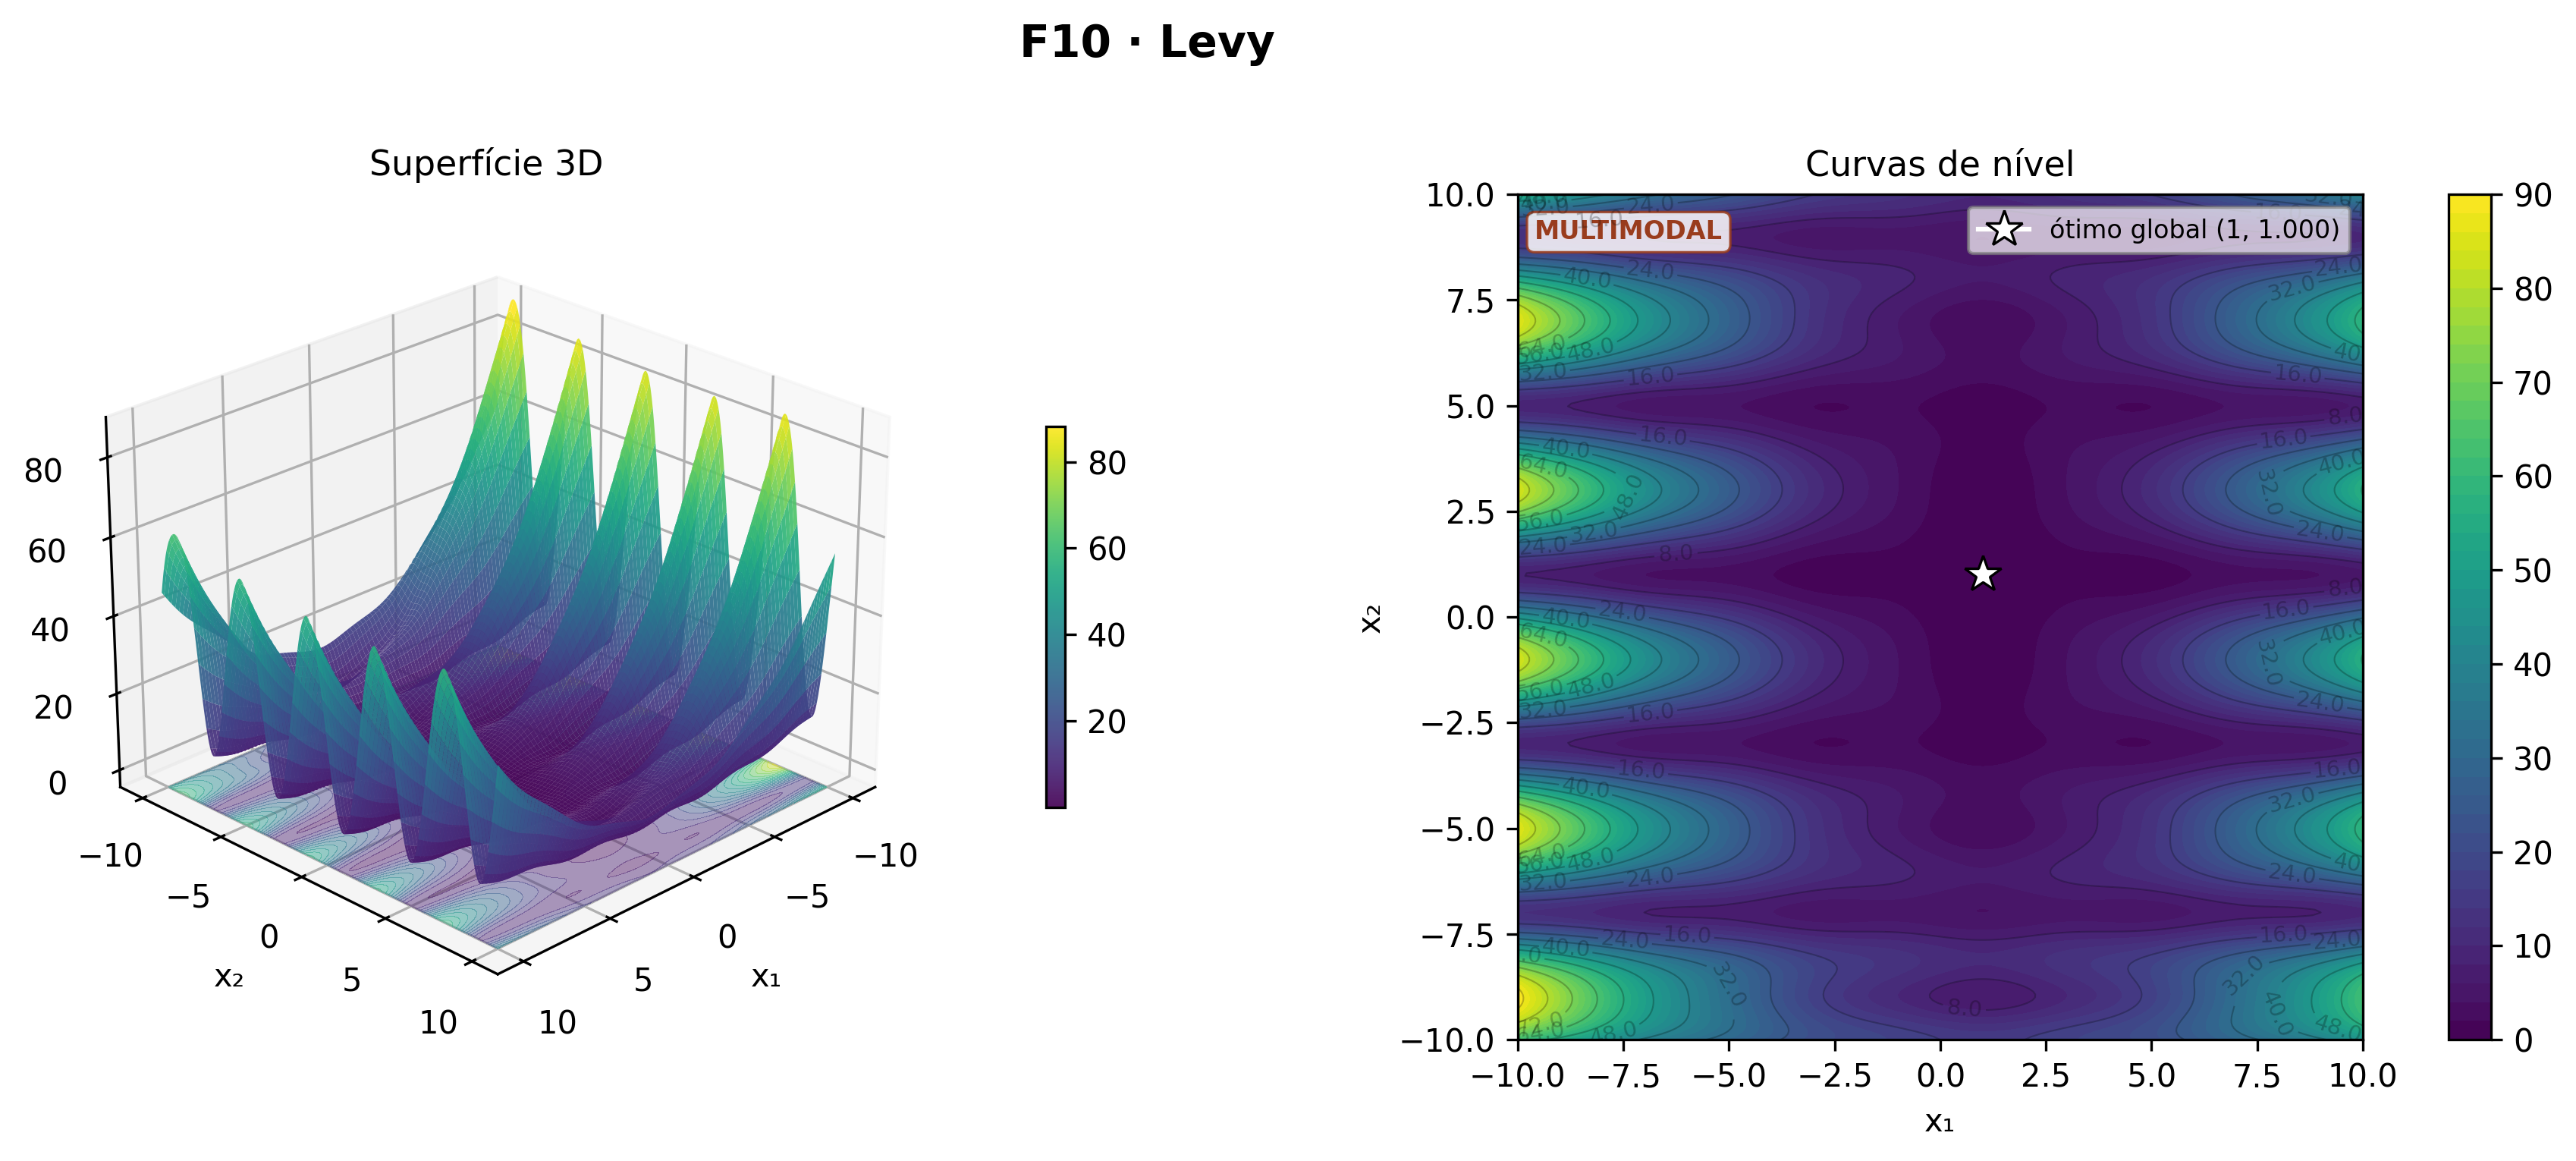
\includegraphics[width=0.75\textwidth]{figs/f10_·_levy.png}
\caption{Superfície 3D e curvas de nível da função Lévy ($D=2$).}
\label{fig:levy}
\end{figure}

%─────────────────────────────────────────────────────────────────────────────
\section{Metodologia}
\label{sec:metodologia}

\subsection{Otimiza\c{c}\~{a}o de Hiperpar\^{a}metros com Optuna}

Os hiperparâmetros de cada algoritmo foram ajustados individualmente
para cada combinação de função e dimensão utilizando o framework
Optuna~\cite{akiba2019} com o amostrador TPE (\emph{Tree-structured
Parzen Estimator}). O TPE modela probabilisticamente as regiões
promissoras do espaço de hiperparâmetros, sendo mais eficiente que
busca aleatória ou em grade para espaços de dimensão moderada.

Para cada combinação (algoritmo, função, dimensão), foram realizados
101~trials. O critério de avaliação de cada trial foi o melhor fitness
obtido ao final de 100.000~avaliações de função, com semente fixa
$s=42$ para reprodutibilidade. O espaço de busca definido para cada
algoritmo foi:

\begin{itemize}
  \item \textbf{AG}: taxa de mutação $p_m \in [0{,}01,\,0{,}20]$,
        desvio $\sigma \in [0{,}05,\,0{,}50]$,
        parâmetro BLX $\alpha \in [0{,}10,\,0{,}50]$.
  \item \textbf{DE}: fator de escala $F \in [0{,}4,\,1{,}5]$,
        taxa de cruzamento $\text{CR} \in [0{,}1,\,1{,}0]$.
  \item \textbf{PSO}: inércia $w \in [0{,}3,\,1{,}0]$,
        coeficientes $c_1, c_2 \in [0{,}5,\,2{,}5]$.
  \item \textbf{EPSO}: probabilidade de comunicação
        $p_c \in [0{,}1,\,0{,}9]$,
        taxa de mutação dos pesos $\tau \in [0{,}05,\,0{,}50]$.
\end{itemize}

Os melhores hiperparâmetros encontrados foram armazenados e utilizados
diretamente na fase experimental, garantindo que cada algoritmo opere
em sua configuração mais favorável para cada cenário.

\subsection{Protocolo Experimental}

O protocolo experimental segue a estrutura adotada por Marcelino
et al.~\cite{marcelino2018}. Para cada combinação de algoritmo,
função e dimensão, foram realizadas 51~execuções independentes com
sementes aleatórias distintas. O único critério de parada é o
esgotamento do orçamento de 100.000~avaliações de função (FEs),
sem critério de convergência antecipada.

O tamanho de população foi fixada em $N=100$ para todos os
algoritmos, essas mesmas configurações foram aplicadas variando a dimensão [30,50,100] garantindo comparação equitativa do custo
por geração. A inicialização é uniforme dentro do domínio de cada
função. As métricas registradas por execução são: melhor fitness
ao final (\emph{best\_f}), número total de avaliações e o
histórico completo de convergência por geração.

A análise estatística adota o Teste~T independente com
$\alpha = 5\%$, hipótese nula de igualdade de médias entre pares
de algoritmos, conforme Marcelino et al.~\cite{marcelino2018}.
Quando a hipótese nula é rejeitada, o vencedor é o algoritmo com
menor média. Quando não é rejeitada, os algoritmos são considerados
estatisticamente equivalentes naquela configuração.

%─────────────────────────────────────────────────────────────────────────────
\section{Resultados e Discuss\~{a}o}
\label{sec:resultados}

Os resultados são apresentados a partir das 51~execuções independentes
por configuração. As tabelas~\ref{tab:unimodais} e~\ref{tab:multimodais}
sintetizam, para cada par (função, dimensão), o algoritmo vencedor com
sua respectiva média e desvio padrão do melhor fitness ao final das
execuções. O melhor resultado de cada linha é destacado em negrito.
As análises subsequentes aprofundam os padrões observados por meio
de visualizações e inferência estatística.

% ── Tabela Unimodais ─────────────────────────────────────────────────────────
\begin{table}[H]
\caption{Melhor resultado por (Função, Dimensão) — Funções Unimodais.
Formato: Média $\pm$ Desvio Padrão.}
\label{tab:unimodais}
\centering
\scriptsize
\begin{tabular}{llll}
\toprule
\textbf{Função} & \textbf{D} & \textbf{Alg.} & $f(\mathbf{x}^*)$ \\
\midrule
\multirow{3}{*}{Sphere}
  & 30  & PSO  & $\mathbf{1{,}60 \times 10^{-89} \pm 1{,}14 \times 10^{-88}}$ \\
  & 50  & PSO  & $\mathbf{9{,}21 \times 10^{-34} \pm 6{,}02 \times 10^{-33}}$ \\
  & 100 & EPSO & $\mathbf{5{,}82 \times 10^{-14} \pm 8{,}11 \times 10^{-14}}$ \\
\midrule
\multirow{3}{*}{Rosenbrock}
  & 30  & PSO  & $\mathbf{1{,}24 \times 10^{1} \pm 1{,}55 \times 10^{1}}$ \\
  & 50  & PSO  & $\mathbf{6{,}94 \times 10^{1} \pm 4{,}14 \times 10^{1}}$ \\
  & 100 & EPSO & $\mathbf{9{,}27 \times 10^{1} \pm 7{,}77 \times 10^{0}}$ \\
\midrule
\multirow{3}{*}{Sum Squares}
  & 30  & PSO  & $\mathbf{4{,}50 \times 10^{-90} \pm 2{,}55 \times 10^{-89}}$ \\
  & 50  & PSO  & $\mathbf{4{,}70 \times 10^{-38} \pm 2{,}62 \times 10^{-37}}$ \\
  & 100 & EPSO & $\mathbf{4{,}57 \times 10^{-14} \pm 1{,}36 \times 10^{-13}}$ \\
\midrule
\multirow{3}{*}{Dixon-Price}
  & 30  & PSO  & $\mathbf{6{,}67 \times 10^{-1} \pm 2{,}24 \times 10^{-16}}$ \\
  & 50  & EPSO & $\mathbf{6{,}67 \times 10^{-1} \pm 1{,}66 \times 10^{-4}}$ \\
  & 100 & EPSO & $\mathbf{6{,}67 \times 10^{-1} \pm 1{,}47 \times 10^{-3}}$ \\
\midrule
\multirow{3}{*}{Zakharov}
  & 30  & EPSO & $\mathbf{1{,}30 \times 10^{-9} \pm 2{,}34 \times 10^{-9}}$ \\
  & 50  & EPSO & $\mathbf{2{,}13 \times 10^{-4} \pm 4{,}08 \times 10^{-4}}$ \\
  & 100 & EPSO & $\mathbf{1{,}86 \times 10^{1} \pm 2{,}21 \times 10^{1}}$ \\
\bottomrule
\end{tabular}
\end{table}

% ── Tabela Multimodais ────────────────────────────────────────────────────────
\begin{table}[H]
\caption{Melhor resultado por (Função, Dimensão) — Funções Multimodais.
Formato: Média $\pm$ Desvio Padrão.}
\label{tab:multimodais}
\centering
\scriptsize
\begin{tabular}{llll}
\toprule
\textbf{Função} & \textbf{D} & \textbf{Alg.} & $f(\mathbf{x}^*)$ \\
\midrule
\multirow{3}{*}{Rastrigin}
  & 30  & DE   & $\mathbf{9{,}97 \times 10^{0} \pm 2{,}43 \times 10^{0}}$ \\
  & 50  & AG   & $\mathbf{2{,}32 \times 10^{1} \pm 4{,}24 \times 10^{0}}$ \\
  & 100 & AG   & $\mathbf{5{,}43 \times 10^{1} \pm 7{,}35 \times 10^{0}}$ \\
\midrule
\multirow{3}{*}{Ackley}
  & 30  & AG   & $\mathbf{4{,}07 \times 10^{-15} \pm 4{,}97 \times 10^{-16}}$ \\
  & 50  & AG   & $\mathbf{1{,}96 \times 10^{-4} \pm 4{,}84 \times 10^{-5}}$ \\
  & 100 & DE   & $\mathbf{2{,}69 \times 10^{-2} \pm 1{,}43 \times 10^{-1}}$ \\
\midrule
\multirow{3}{*}{Griewank}
  & 30  & DE   & $\mathbf{4{,}02 \times 10^{-15} \pm 1{,}51 \times 10^{-14}}$ \\
  & 50  & DE   & $\mathbf{5{,}80 \times 10^{-4} \pm 2{,}49 \times 10^{-3}}$ \\
  & 100 & EPSO & $\mathbf{2{,}57 \times 10^{-3} \pm 5{,}67 \times 10^{-3}}$ \\
\midrule
\multirow{3}{*}{Schwefel 2.26}
  & 30  & AG   & $\mathbf{-1{,}14 \times 10^{53} \pm 8{,}15 \times 10^{53}}$ \\
  & 50  & AG   & $\mathbf{-4{,}92 \times 10^{41} \pm 2{,}42 \times 10^{42}}$ \\
  & 100 & AG   & $\mathbf{-1{,}17 \times 10^{46} \pm 8{,}25 \times 10^{46}}$ \\
\midrule
\multirow{3}{*}{Lévy}
  & 30  & AG   & $\mathbf{8{,}00 \times 10^{-30} \pm 5{,}44 \times 10^{-29}}$ \\
  & 50  & DE   & $\mathbf{1{,}16 \times 10^{-13} \pm 1{,}37 \times 10^{-13}}$ \\
  & 100 & DE   & $\mathbf{5{,}63 \times 10^{-6} \pm 3{,}09 \times 10^{-6}}$ \\
\bottomrule
\end{tabular}
\end{table}

\subsection{Curvas de Converg\^{e}ncia M\'{e}dia}

As curvas de convergência média são obtidas pela interpolação das 51
trajetórias de cada execução em uma grade comum de FEs, seguida do
cálculo da média ponto a ponto. O eixo $x$ representa as avaliações
acumuladas de função e o eixo $y$ utiliza escala simlog para capturar
ordens de magnitude distintas sem perda de informação próximo ao zero.

% ── curvas de convergência ────────────────────────────────────────────────────
\begin{figure}[H]
\centering
\begin{subfigure}{\textwidth}
  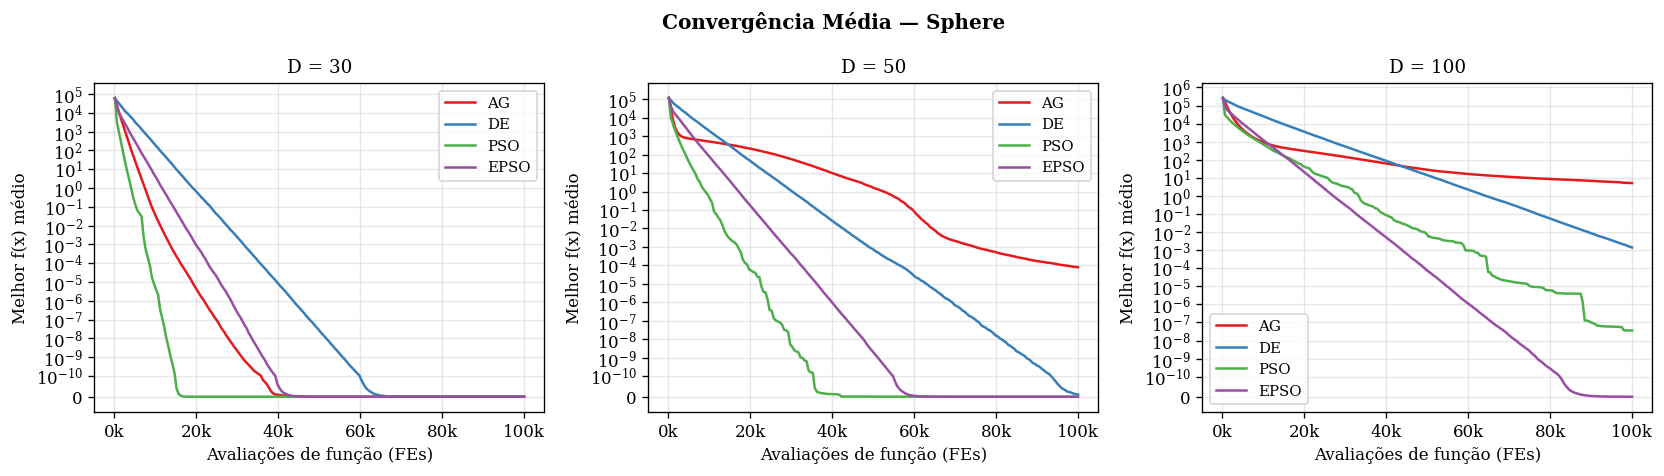
\includegraphics[width=\textwidth]{figs/conv_sphere.png}
  \caption{Sphere}
\end{subfigure}
\begin{subfigure}{\textwidth}
  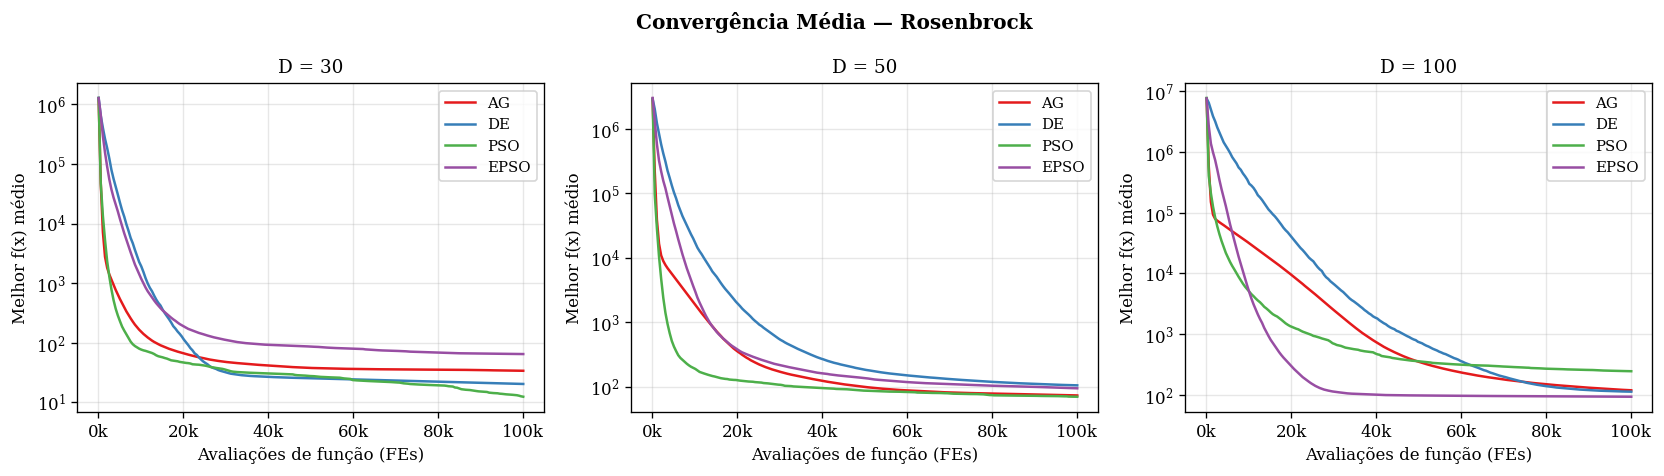
\includegraphics[width=\textwidth]{figs/conv_rosenbrock.png}
  \caption{Rosenbrock}
\end{subfigure}
\begin{subfigure}{\textwidth}
  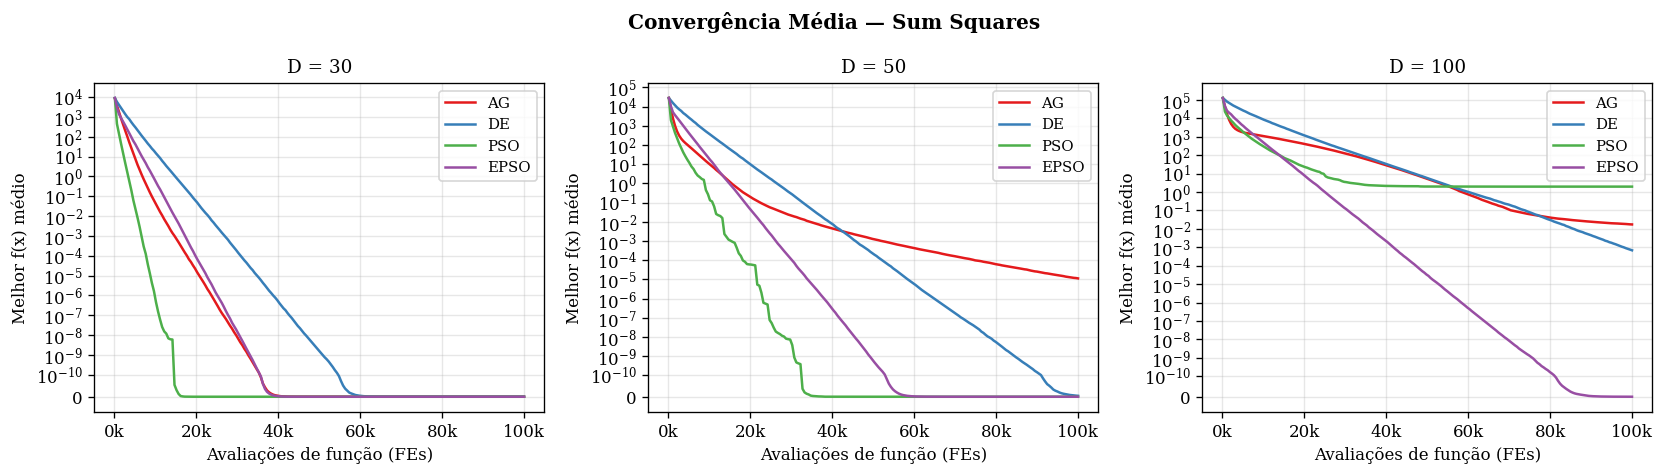
\includegraphics[width=\textwidth]{figs/conv_sum_squares.png}
  \caption{Sum Squares}
\end{subfigure}
\begin{subfigure}{\textwidth}
  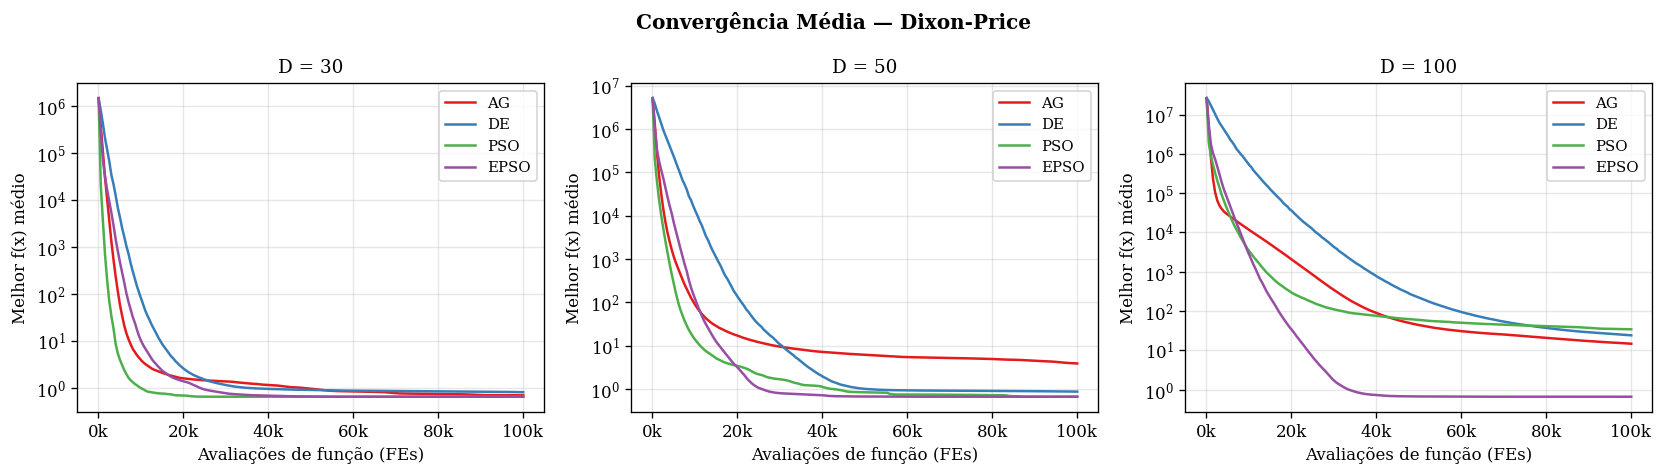
\includegraphics[width=\textwidth]{figs/conv_dixon_price.png}
  \caption{Dixon-Price}
\end{subfigure}
\begin{subfigure}{\textwidth}
  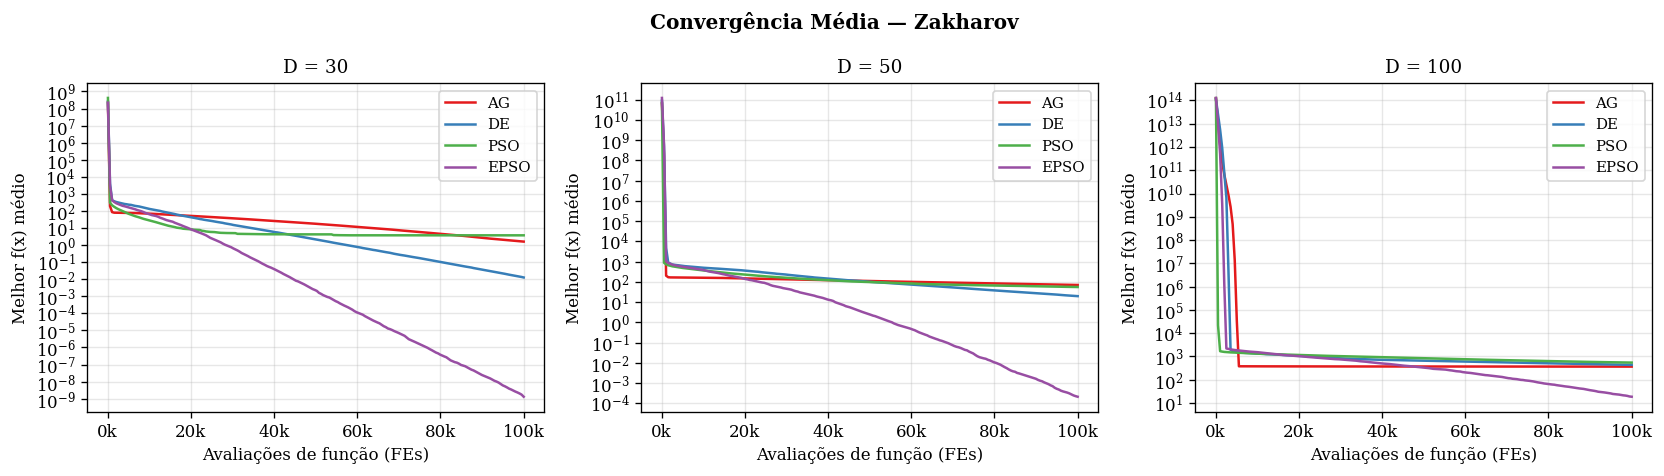
\includegraphics[width=\textwidth]{figs/conv_zakharov.png}
  \caption{Zakharov}
\end{subfigure}
\caption{Curvas de convergência média para as dez funções benchmark unimodais nas dimensões 30, 50 e~100.}
\label{fig:conv_unimodais}
\end{figure}

\begin{figure}[H]
\centering
\begin{subfigure}{\textwidth}
  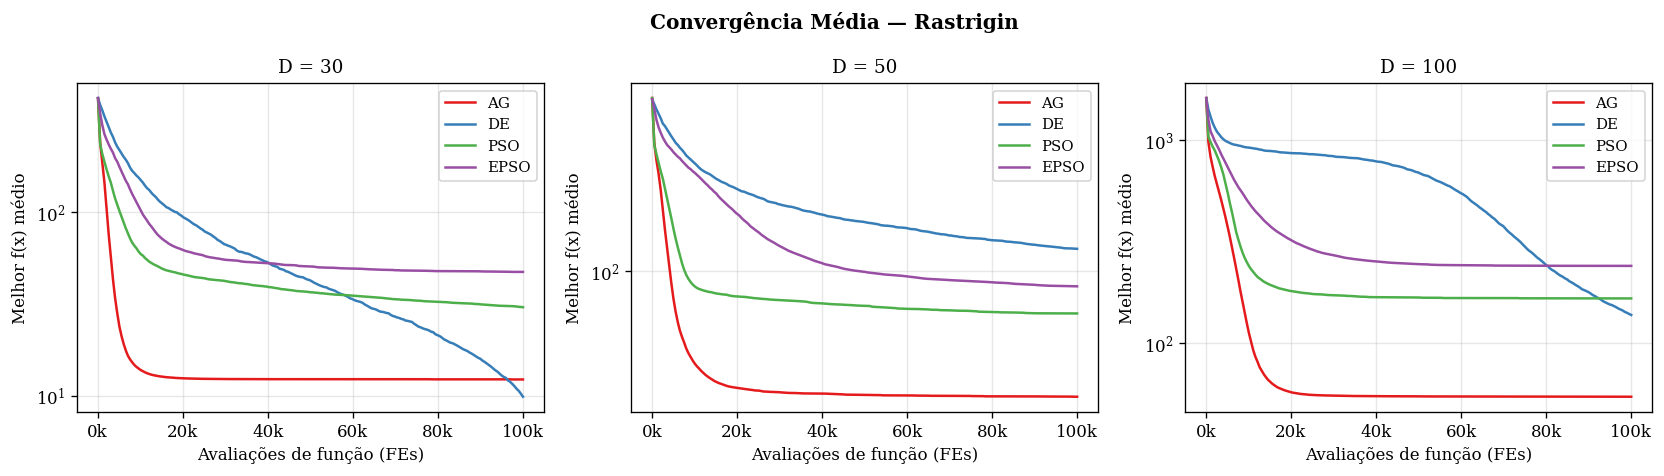
\includegraphics[width=\textwidth]{figs/conv_rastrigin.png}
  \caption{Rastrigin}
\end{subfigure}
\begin{subfigure}{\textwidth}
  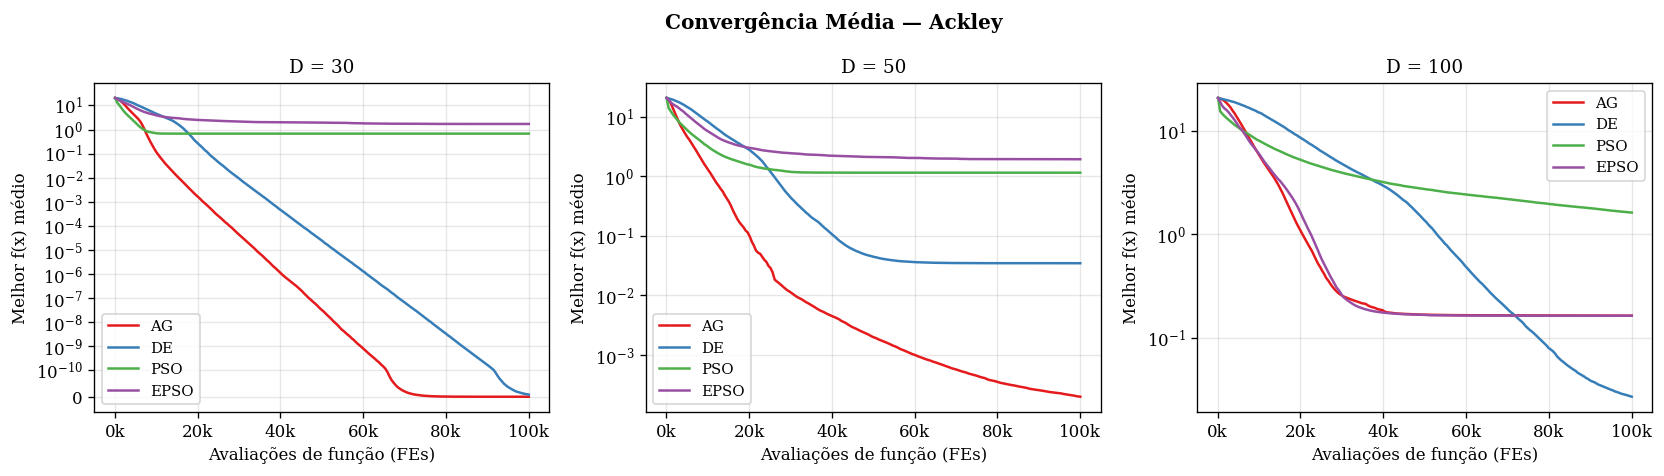
\includegraphics[width=\textwidth]{figs/conv_ackley.png}
  \caption{Ackley}
\end{subfigure}
\begin{subfigure}{\textwidth}
  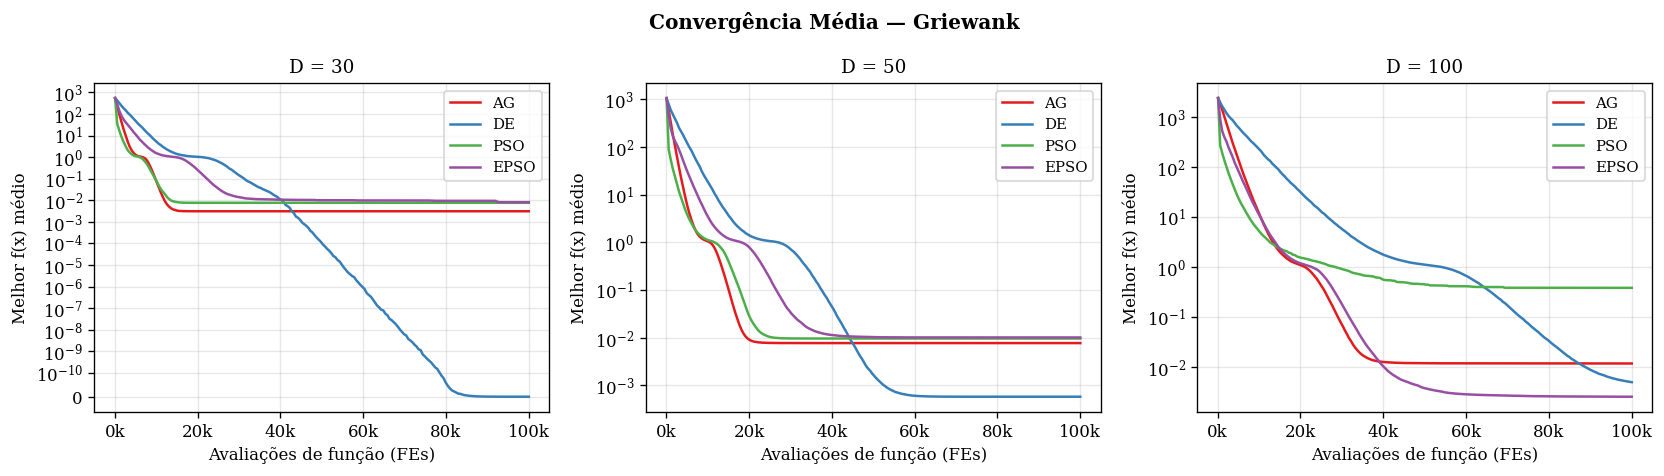
\includegraphics[width=\textwidth]{figs/conv_griewank.png}
  \caption{Griewank}
\end{subfigure}
\begin{subfigure}{\textwidth}
  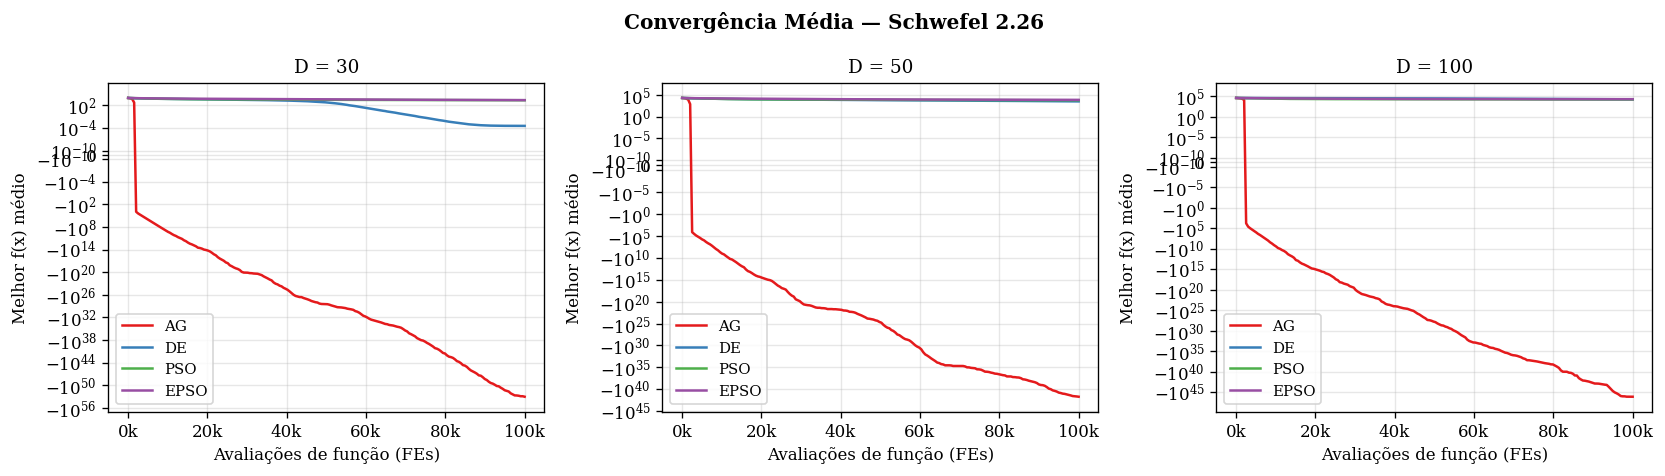
\includegraphics[width=\textwidth]{figs/conv_schwefel.png}
  \caption{Schwefel 2.26}
\end{subfigure}
\begin{subfigure}{\textwidth}
  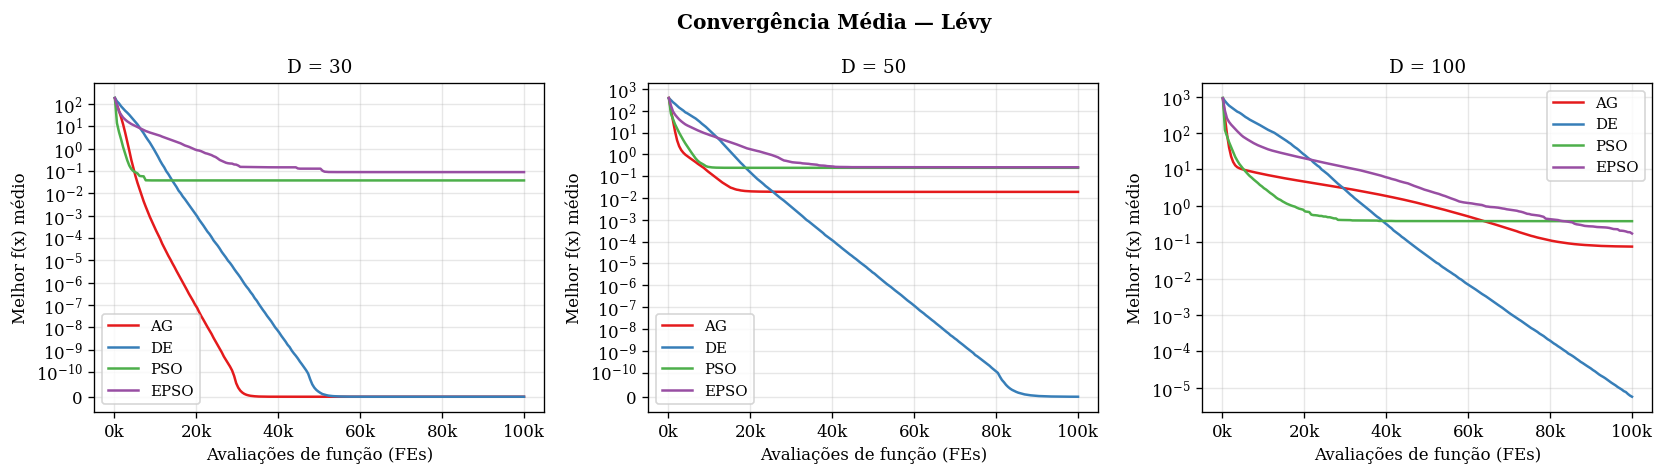
\includegraphics[width=\textwidth]{figs/conv_levy.png}
  \caption{Lévy}
\end{subfigure}
\caption{Curvas de convergência média para as dez funções benchmark multimodais nas dimensões 30, 50 e~100.}
\label{fig:conv_multimodais}
\end{figure}

Nas funções unimodais separáveis, como Sphere e Sum Squares, PSO e
EPSO tendem a apresentar convergência rápida nas dimensões menores,
beneficiando-se da estrutura separável que permite atualização
independente por dimensão. Em Rosenbrock, o vale estreito e curvo
penaliza algoritmos que não coordenam dimensões adjacentes, favorecendo
DE pela natureza da mutação diferencial. À medida que $D$ aumenta
para 100, a velocidade de convergência de todos os algoritmos diminui,
com AG apresentando a degradação mais pronunciada.

Nas funções multimodais, a densidade de ótimos locais de Rastrigin
e o caráter deceptivo de Schwefel 2.26 criam comportamentos
qualitativamente distintos. Algoritmos que mantêm diversidade
populacional por mais gerações tendem a encontrar melhores soluções
finais, ainda que a convergência seja mais lenta no início.

\subsection{Boxplots}

Os boxplots da Figura~\ref{fig:boxplots} apresentam a distribuição
das 51~execuções para Rosenbrock, Rastrigin, Zakharov e Schwefel~2.26
nas três dimensões. A largura de cada caixa e a presença de outliers
revelam a estabilidade de cada algoritmo além da média reportada nas
tabelas.

\begin{figure}[htbp]
\centering
\begin{subfigure}{\textwidth}
  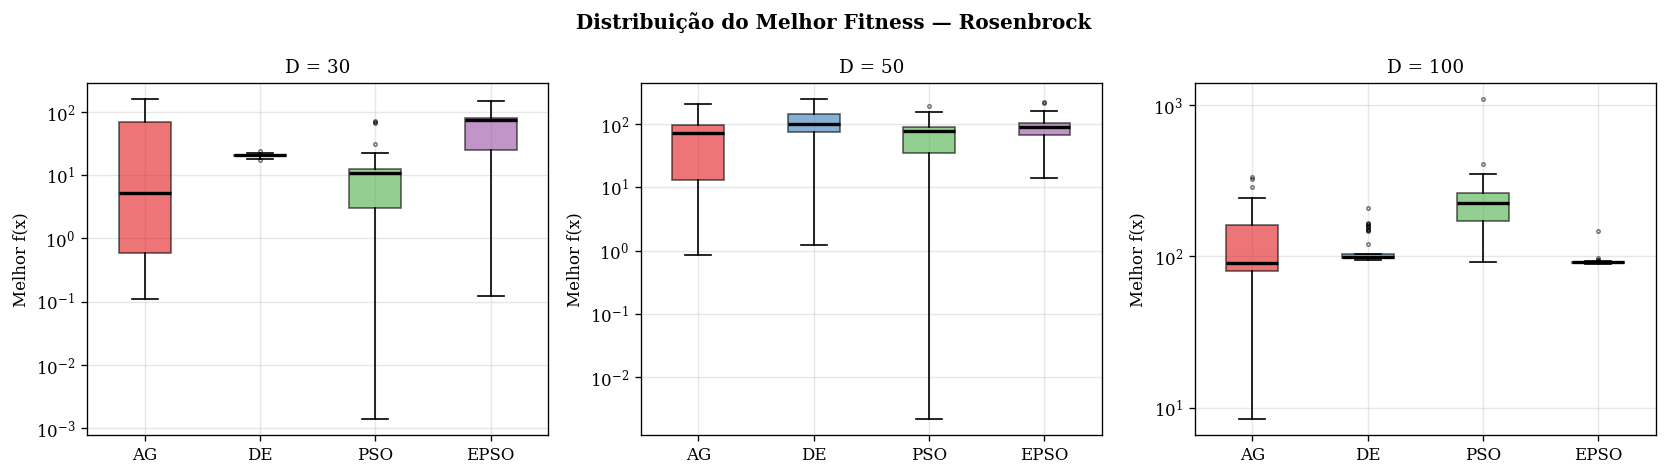
\includegraphics[width=\textwidth]{figs/box_rosenbrock.png}
  \caption{Rosenbrock}
\end{subfigure}
\begin{subfigure}{\textwidth}
  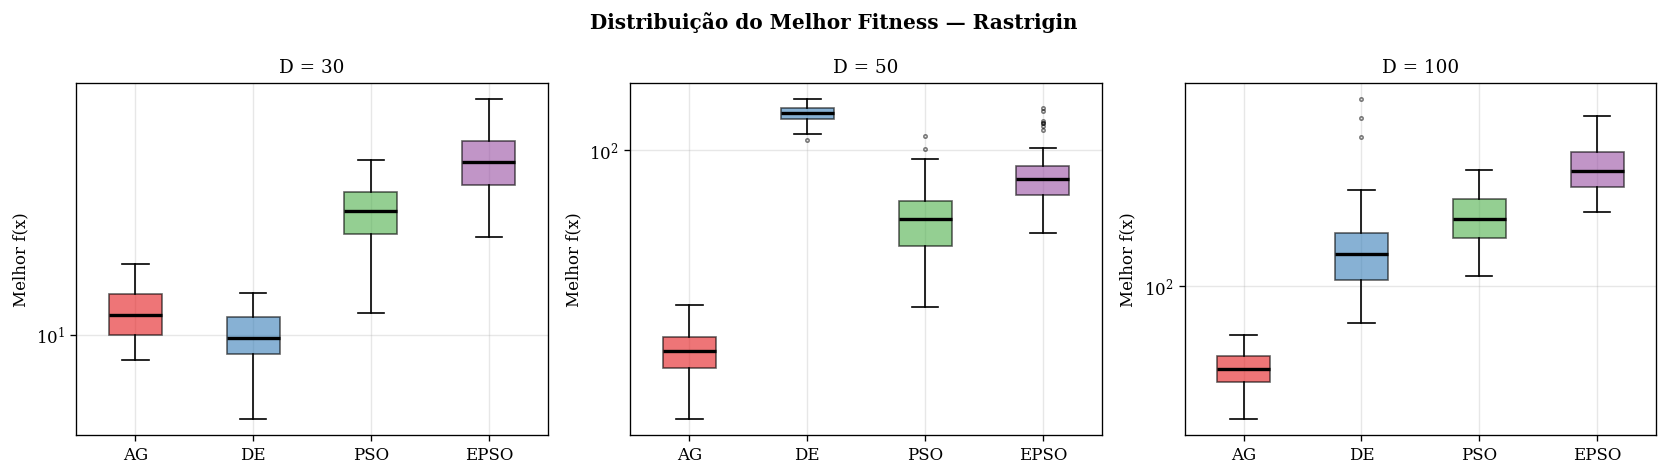
\includegraphics[width=\textwidth]{figs/box_rastrigin.png}
  \caption{Rastrigin}
\end{subfigure}
\caption{Distribuição do melhor fitness nas 51~execuções — Rosenbrock e Rastrigin.}
\label{fig:boxplots_a}
\end{figure}

\begin{figure}[htbp]
\centering
\begin{subfigure}{\textwidth}
  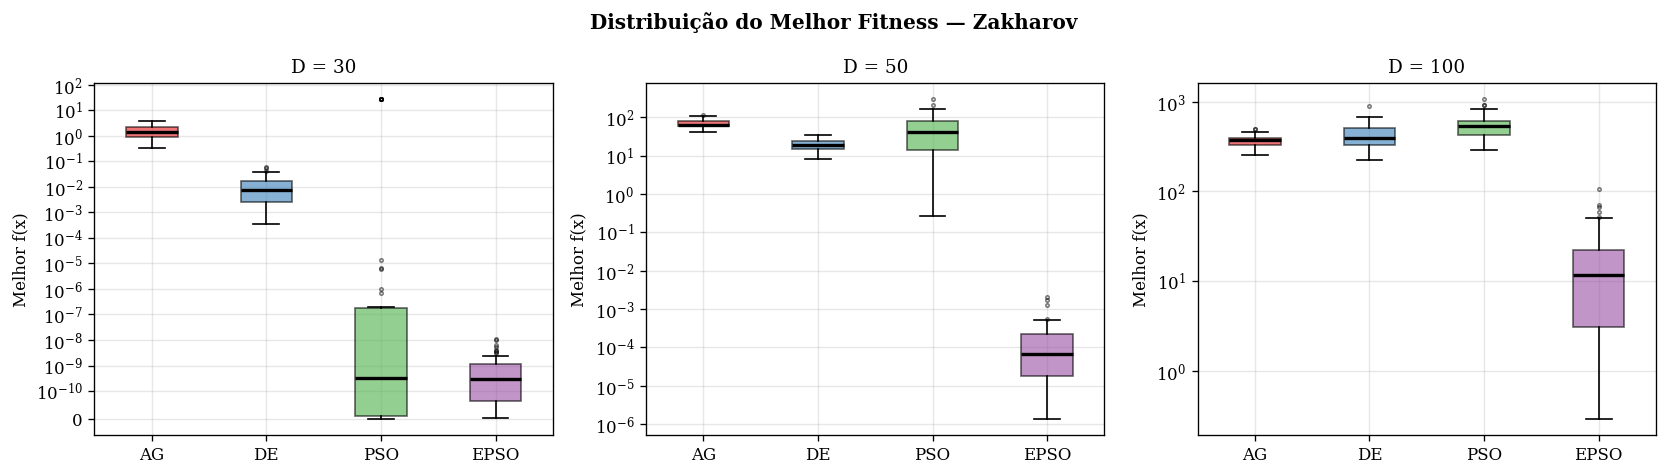
\includegraphics[width=\textwidth]{figs/box_zakharov.png}
  \caption{Zakharov}
\end{subfigure}
\begin{subfigure}{\textwidth}
  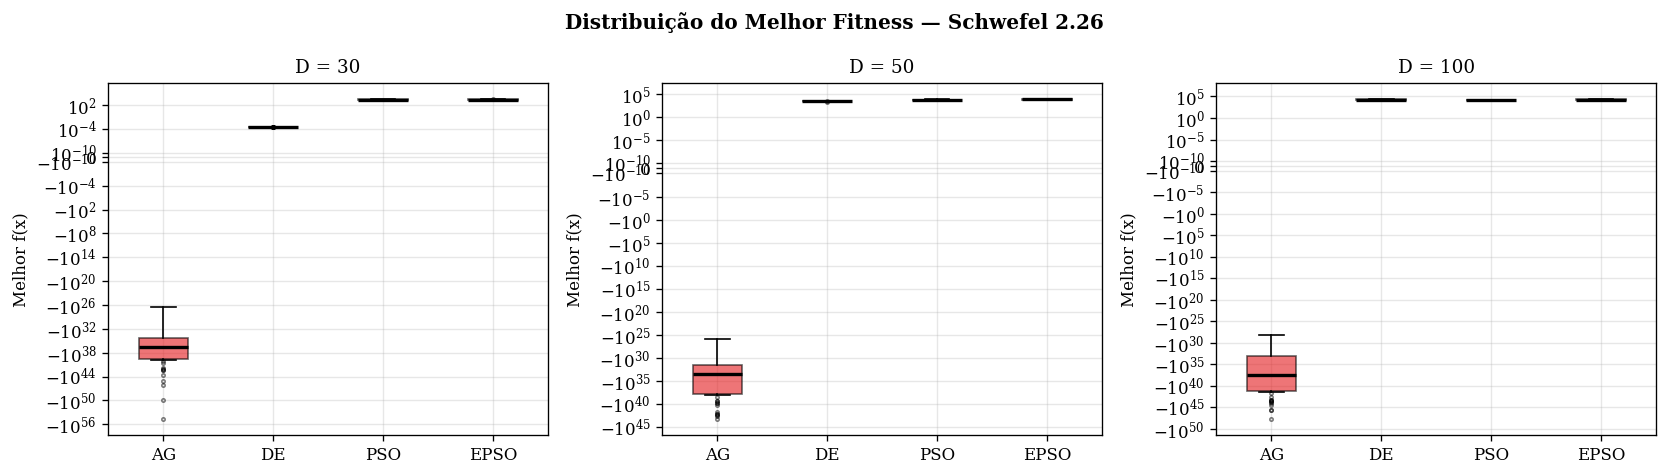
\includegraphics[width=\textwidth]{figs/box_schwefel.png}
  \caption{Schwefel 2.26}
\end{subfigure}
\caption{Distribuição do melhor fitness nas 51~execuções — Zakharov e Schwefel 2.26.
Linha central: mediana; caixa: IQR; pontos: outliers.}
\label{fig:boxplots}
\end{figure}

Algoritmos com caixas estreitas e poucos outliers são mais robustos —
seus resultados dependem menos da inicialização aleatória. Caixas
largas indicam alta sensibilidade à semente, especialmente em funções
multimodais onde diferentes execuções podem convergir para distintos
ótimos locais. Em Schwefel~2.26, espera-se observar outliers extremos
para algoritmos que não localizam o ótimo global periférico na maioria
das execuções.

\subsection{An\'{a}lise Estat\'{i}stica}

A significância estatística das diferenças observadas é avaliada
primariamente pelo Teste~T de Welch para amostras independentes
($\alpha = 5\%$), seguindo Marcelino et al.~\cite{marcelino2018}.
A hipótese nula $H_0\!: \mu_1 = \mu_2$ é testada para cada par de
algoritmos, por função e dimensão. Quando $H_0$ é rejeitada
($p < 0{,}05$), o vencedor é identificado como o algoritmo de menor
média. Quando não é rejeitada, reporta-se equivalência estatística
entre os dois algoritmos naquela configuração.

Como análise complementar, aplica-se o teste de Wilcoxon
Rank-Sum (Mann-Whitney~U), não-paramétrico e robusto a distribuições
assimétricas e outliers, com o vencedor determinado pela menor
mediana. A comparação entre os dois testes permite identificar casos
onde a presença de valores extremos influencia as conclusões do
Teste~T\@. Importa notar que em configurações onde múltiplos
algoritmos convergem para valores próximos da precisão numérica de
\textit{float64} (por exemplo, Sphere em $D=30$), o Teste~T pode
apresentar cancelamento catastrófico na estimativa da variância,
tornando-o conservador nesses casos específicos. O Wilcoxon, por
operar sobre ranks, é imune a esse efeito.

A Tabela~\ref{tab:ranking_t} sumariza o ranking consolidado de
vitórias de cada teste ao longo de todas as combinações
função~$\times$~dimensão
($6\ \text{pares} \times 30\ \text{configurações} = 180\ \text{testes}$).

\begin{table}[H]
\caption{Ranking consolidado de vitórias ($\alpha = 5\%$) por teste
estatístico. Teste~T de Welch (vencedor = menor média);
Wilcoxon Rank-Sum (vencedor = menor mediana).}
\label{tab:ranking_t}
\centering
\begin{tabular}{lcccc}
\toprule
\textbf{Teste} & \textbf{AG} & \textbf{DE} & \textbf{PSO} & \textbf{EPSO} \\
\midrule
Teste T de Welch  & 31 & \textbf{40} & 24 & 29 \\
Wilcoxon Rank-Sum & 39 & 34 & \textbf{45} & 39 \\
\bottomrule
\end{tabular}
\end{table}

A divergência entre os dois testes concentra-se nas funções onde
algoritmos atingem valores próximos de zero (Sphere, Sum~Squares),
nas quais o Wilcoxon detecta diferenças que o Teste~T deixa escapar
por instabilidade numérica. Nas funções multimodais, onde as
distribuições de fitness são mais espalhadas e assimétricas, os dois
testes convergem para as mesmas conclusões na maioria dos pares.

\subsection{An\'{a}lise de Escalabilidade}

A análise de escalabilidade examina como o desempenho de cada algoritmo
se degrada com o aumento da dimensão de $D=30$ para $D=100$.
A Figura~\ref{fig:escalabilidade} apresenta a evolução da mediana do
fitness por algoritmo e função.

\begin{figure}[htbp]
\centering
\begin{subfigure}{\textwidth}
  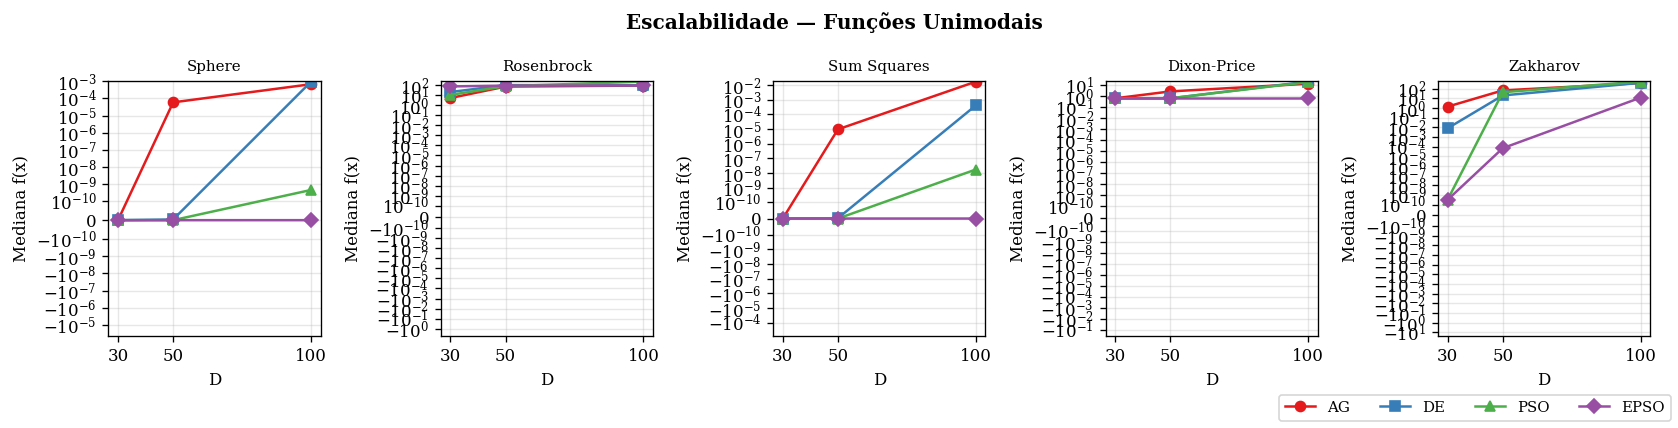
\includegraphics[width=\textwidth]{figs/escal_unimodais.png}
  \caption{Funções unimodais}
\end{subfigure}
\begin{subfigure}{\textwidth}
  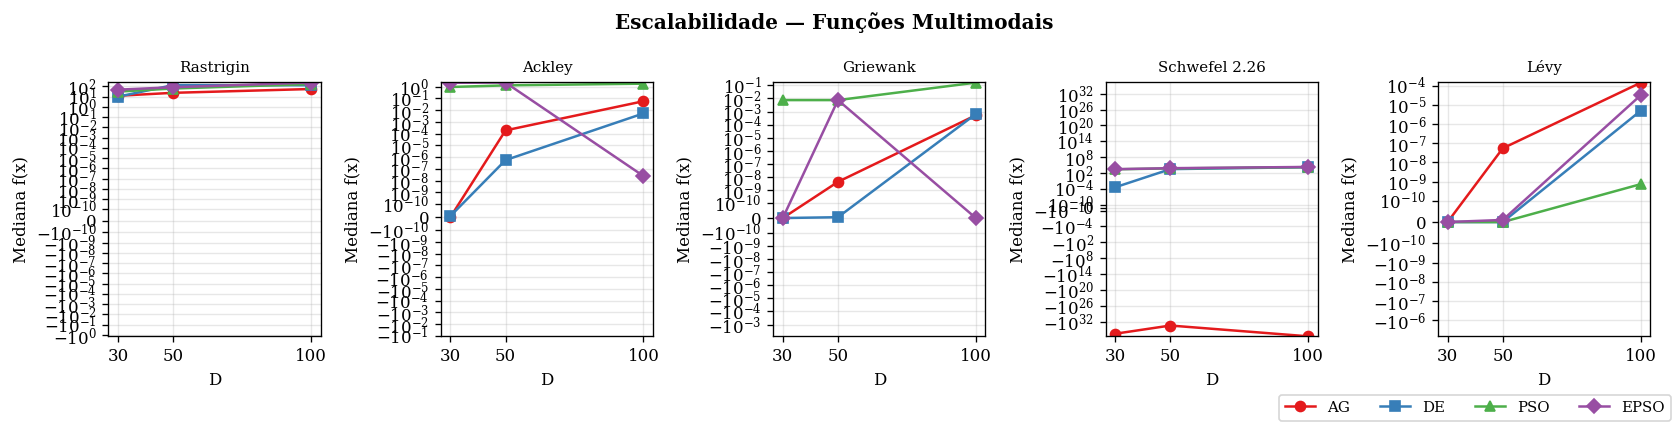
\includegraphics[width=\textwidth]{figs/escal_multimodais.png}
  \caption{Funções multimodais}
\end{subfigure}
\caption{Escalabilidade: mediana do fitness em função da dimensão
($D \in \{30, 50, 100\}$) para cada algoritmo e função benchmark.
Escala $y$ simlog.}
\label{fig:escalabilidade}
\end{figure}

Funções não-separáveis como Rosenbrock e Zakharov tendem a apresentar
degradação mais severa para todos os algoritmos, uma vez que a
interação entre dimensões amplifica a dificuldade do problema à medida
que $D$ cresce. Entre os algoritmos, espera-se que aqueles com
mecanismos de adaptação (EPSO) mantenham desempenho relativo mais
estável em alta dimensão em comparação ao AG, que não possui mecanismo
de auto-adaptação de passo.

\subsection{Velocidade de Converg\^{e}ncia}

A velocidade de convergência é quantificada pela Área sob a Curva
(AUC) de convergência, calculada como a integral numérica de
$f_{\text{best}}$ ao longo dos FEs usando a regra do trapézio.
Um valor menor de AUC indica que o algoritmo acumulou valores baixos
de fitness mais cedo durante o processo de busca, independentemente
do valor final atingido.

A Tabela~\ref{tab:auc} apresenta a mediana da AUC por algoritmo,
função e dimensão, com o algoritmo mais rápido destacado em verde.

\begin{table}[H]
\caption{AUC das curvas de convergência médias por algoritmo e função.
Menor AUC indica convergência mais rápida acumulada. Melhor valor por
linha em negrito com fundo verde.}
\label{tab:auc}
\centering
\scriptsize
\setlength{\tabcolsep}{4pt}
\begin{tabular}{llccccc}
\toprule
\textbf{Função} & \textbf{D} &
\textbf{AG} & \textbf{DE} & \textbf{PSO} & \textbf{EPSO} & \textbf{Melhor} \\
\midrule
% ── UNIMODAIS ────────────────────────────────────────────────────────────────
\multirow{3}{*}{Sphere}
  & 30  & $3{,}54{\times}10^{7}$ & $9{,}75{\times}10^{7}$ & \cellcolor{green!20}$\mathbf{8{,}67{\times}10^{6}}$ & $3{,}80{\times}10^{7}$ & PSO \\
  & 50  & $5{,}03{\times}10^{7}$ & $2{,}43{\times}10^{8}$ & \cellcolor{green!20}$\mathbf{2{,}26{\times}10^{7}}$ & $8{,}30{\times}10^{7}$ & PSO \\
  & 100 & $2{,}68{\times}10^{8}$ & $9{,}96{\times}10^{8}$ & \cellcolor{green!20}$\mathbf{1{,}01{\times}10^{8}}$ & $2{,}46{\times}10^{8}$ & PSO \\
\midrule
\multirow{3}{*}{Rosenbrock}
  & 30  & $1{,}99{\times}10^{8}$ & $1{,}27{\times}10^{9}$ & \cellcolor{green!20}$\mathbf{1{,}47{\times}10^{8}}$ & $9{,}96{\times}10^{8}$ & PSO \\
  & 50  & $6{,}43{\times}10^{8}$ & $3{,}89{\times}10^{9}$ & \cellcolor{green!20}$\mathbf{3{,}45{\times}10^{8}}$ & $2{,}23{\times}10^{9}$ & PSO \\
  & 100 & $2{,}24{\times}10^{9}$ & $2{,}06{\times}10^{10}$ & \cellcolor{green!20}$\mathbf{1{,}33{\times}10^{9}}$ & $5{,}37{\times}10^{9}$ & PSO \\
\midrule
\multirow{3}{*}{Sum Squares}
  & 30  & $5{,}47{\times}10^{6}$ & $1{,}21{\times}10^{7}$ & \cellcolor{green!20}$\mathbf{1{,}24{\times}10^{6}}$ & $5{,}24{\times}10^{6}$ & PSO \\
  & 50  & $1{,}21{\times}10^{7}$ & $5{,}35{\times}10^{7}$ & \cellcolor{green!20}$\mathbf{4{,}89{\times}10^{6}}$ & $2{,}03{\times}10^{7}$ & PSO \\
  & 100 & $8{,}44{\times}10^{7}$ & $4{,}09{\times}10^{8}$ & \cellcolor{green!20}$\mathbf{5{,}96{\times}10^{7}}$ & $1{,}11{\times}10^{8}$ & PSO \\
\midrule
\multirow{3}{*}{Dixon-Price}
  & 30  & $5{,}51{\times}10^{8}$ & $1{,}26{\times}10^{9}$ & \cellcolor{green!20}$\mathbf{1{,}36{\times}10^{8}}$ & $5{,}36{\times}10^{8}$ & PSO \\
  & 50  & $1{,}89{\times}10^{9}$ & $8{,}10{\times}10^{9}$ & \cellcolor{green!20}$\mathbf{6{,}11{\times}10^{8}}$ & $1{,}96{\times}10^{9}$ & PSO \\
  & 100 & $8{,}09{\times}10^{9}$ & $5{,}97{\times}10^{10}$ & \cellcolor{green!20}$\mathbf{4{,}92{\times}10^{9}}$ & $1{,}02{\times}10^{10}$ & PSO \\
\midrule
\multirow{3}{*}{Zakharov}
  & 30  & \cellcolor{green!20}$\mathbf{1{,}94{\times}10^{9}}$ & $3{,}44{\times}10^{9}$ & $1{,}58{\times}10^{10}$ & $4{,}08{\times}10^{9}$ & AG \\
  & 50  & $5{,}27{\times}10^{12}$ & $6{,}92{\times}10^{12}$ & \cellcolor{green!20}$\mathbf{4{,}20{\times}10^{12}}$ & $7{,}28{\times}10^{12}$ & PSO \\
  & 100 & $2{,}55{\times}10^{16}$ & $3{,}33{\times}10^{16}$ & \cellcolor{green!20}$\mathbf{2{,}15{\times}10^{16}}$ & $2{,}21{\times}10^{16}$ & PSO \\
\midrule
% ── MULTIMODAIS ──────────────────────────────────────────────────────────────
\multirow{3}{*}{Rastrigin}
  & 30  & \cellcolor{green!20}$\mathbf{1{,}72{\times}10^{6}}$ & $6{,}64{\times}10^{6}$ & $4{,}55{\times}10^{6}$ & $6{,}47{\times}10^{6}$ & AG \\
  & 50  & \cellcolor{green!20}$\mathbf{3{,}63{\times}10^{6}}$ & $2{,}16{\times}10^{7}$ & $8{,}04{\times}10^{6}$ & $1{,}49{\times}10^{7}$ & AG \\
  & 100 & \cellcolor{green!20}$\mathbf{9{,}55{\times}10^{6}}$ & $5{,}95{\times}10^{7}$ & $2{,}11{\times}10^{7}$ & $3{,}10{\times}10^{7}$ & AG \\
\midrule
\multirow{3}{*}{Ackley}
  & 30  & \cellcolor{green!20}$\mathbf{6{,}04{\times}10^{4}}$ & $1{,}39{\times}10^{5}$ & $1{,}20{\times}10^{5}$ & $2{,}96{\times}10^{5}$ & AG \\
  & 50  & \cellcolor{green!20}$\mathbf{7{,}20{\times}10^{4}}$ & $2{,}12{\times}10^{5}$ & $1{,}91{\times}10^{5}$ & $3{,}44{\times}10^{5}$ & AG \\
  & 100 & $1{,}70{\times}10^{5}$ & $4{,}37{\times}10^{5}$ & $3{,}96{\times}10^{5}$ & \cellcolor{green!20}$\mathbf{1{,}58{\times}10^{5}}$ & EPSO \\
\midrule
\multirow{3}{*}{Griewank}
  & 30  & $3{,}23{\times}10^{5}$ & $1{,}10{\times}10^{6}$ & \cellcolor{green!20}$\mathbf{9{,}93{\times}10^{4}}$ & $5{,}18{\times}10^{5}$ & PSO \\
  & 50  & $9{,}14{\times}10^{5}$ & $2{,}30{\times}10^{6}$ & \cellcolor{green!20}$\mathbf{2{,}57{\times}10^{5}}$ & $9{,}99{\times}10^{5}$ & PSO \\
  & 100 & $4{,}20{\times}10^{6}$ & $8{,}90{\times}10^{6}$ & \cellcolor{green!20}$\mathbf{8{,}59{\times}10^{5}}$ & $2{,}20{\times}10^{6}$ & PSO \\
\midrule
\multirow{3}{*}{Schwefel 2.26}
  & 30  & \cellcolor{green!20}$\mathbf{-6{,}51{\times}10^{39}}$ & $1{,}96{\times}10^{8}$ & $3{,}68{\times}10^{8}$ & $4{,}53{\times}10^{8}$ & AG \\
  & 50  & \cellcolor{green!20}$\mathbf{-5{,}10{\times}10^{36}}$ & $6{,}35{\times}10^{8}$ & $7{,}22{\times}10^{8}$ & $9{,}12{\times}10^{8}$ & AG \\
  & 100 & \cellcolor{green!20}$\mathbf{-1{,}29{\times}10^{41}}$ & $2{,}80{\times}10^{9}$ & $1{,}90{\times}10^{9}$ & $2{,}23{\times}10^{9}$ & AG \\
\midrule
\multirow{3}{*}{Lévy}
  & 30  & $1{,}37{\times}10^{5}$ & $3{,}59{\times}10^{5}$ & \cellcolor{green!20}$\mathbf{3{,}20{\times}10^{4}}$ & $2{,}10{\times}10^{5}$ & PSO \\
  & 50  & $1{,}62{\times}10^{5}$ & $1{,}01{\times}10^{6}$ & \cellcolor{green!20}$\mathbf{1{,}36{\times}10^{5}}$ & $4{,}58{\times}10^{5}$ & PSO \\
  & 100 & $6{,}31{\times}10^{5}$ & $4{,}49{\times}10^{6}$ & \cellcolor{green!20}$\mathbf{3{,}78{\times}10^{5}}$ & $1{,}72{\times}10^{6}$ & PSO \\
\midrule
\multicolumn{2}{l}{\textbf{Ranking (vitórias AUC)}} & & & & & \\
\multicolumn{2}{l}{$D=30$}  & 4 & 0 & \textbf{6} & 0 & \\
\multicolumn{2}{l}{$D=50$}  & 3 & 0 & \textbf{7} & 0 & \\
\multicolumn{2}{l}{$D=100$} & 2 & 0 & \textbf{7} & 1 & \\
\bottomrule
\multicolumn{7}{l}{\scriptsize $^\dagger$AUC negativa em Schwefel~2.26 (AG): fitness negativo
  por construção da função deslocada.}
\end{tabular}
\end{table}

%─────────────────────────────────────────────────────────────────────────────
\section{Conclus\~{a}o}
\label{sec:conclusao}

Este trabalho apresentou uma comparação sistemática entre AG, DE, PSO
e EPSO em dez funções benchmark escaláveis, nas dimensões 30, 50 e
100, com hiperparâmetros ajustados individualmente via Optuna e
protocolo experimental com 51~execuções independentes.

Os resultados indicam que nenhum algoritmo domina em todos os cenários.
Em funções unimodais separáveis, PSO e EPSO destacam-se pela velocidade
de convergência nas dimensões menores, enquanto DE demonstra vantagem
em funções com estrutura não-separável como Rosenbrock. Em funções
multimodais, a capacidade de manter diversidade populacional ao longo
das avaliações mostra-se determinante, com comportamentos distintos
entre as funções de acordo com a densidade e a localização dos ótimos
locais. A análise de escalabilidade revela que todos os algoritmos
sofrem degradação de desempenho com o aumento de dimensão, mas em
graus variáveis conforme o tipo de função.

Como limitações, o estudo utiliza funções benchmark clássicas sem
ruído e adota tamanho de população fixo em todos os cenários. Trabalhos
futuros incluem a extensão para DEEPSO e C-DEEPSO~\cite{marcelino2018}.


%─────────────────────────────────────────────────────────────────────────────
\begin{thebibliography}{9}

\bibitem{goldberg1989}
Goldberg, D.E.: Genetic Algorithms in Search, Optimization and
Machine Learning. Addison-Wesley, Reading, MA (1989)

\bibitem{storn1997}
Storn, R., Price, K.: Differential evolution -- a simple and efficient
heuristic for global optimization over continuous spaces.
Journal of Global Optimization \textbf{11}(4), 341--359 (1997).
\doi{10.1023/A:1008202821328}

\bibitem{kennedy1995}
Kennedy, J., Eberhart, R.: Particle swarm optimization.
In: Proceedings of the IEEE International Conference on Neural
Networks, vol.~4, pp.~1942--1948. IEEE, Perth (1995).
\doi{10.1109/ICNN.1995.488968}

\bibitem{miranda2002}
Miranda, V., Fonseca, N.: EPSO -- evolutionary particle swarm
optimization, a new algorithm with applications in power systems.
In: Proceedings of the IEEE/PES Transmission and Distribution
Conference and Exhibition, vol.~2, pp.~745--750. IEEE (2002).
\doi{10.1109/TDC.2002.1177567}

\bibitem{marcelino2018}
Marcelino, C.G., Almeida, P.E.M., Wanner, E.F., Baumann, M.,
Weil, M., Carvalho, L.M., Miranda, V.: Solving security constrained
optimal power flow problems: a hybrid evolutionary approach.
Applied Intelligence \textbf{48}(10), 3672--3690 (2018).
\doi{10.1007/s10489-018-1167-5}

\bibitem{akiba2019}
Akiba, T., Sano, S., Yanase, T., Ohta, T., Koyama, M.:
Optuna: A next-generation hyperparameter optimization framework.
In: Proceedings of the 25th ACM SIGKDD International Conference on
Knowledge Discovery \& Data Mining, pp.~2623--2631. ACM (2019).
\doi{10.1145/3292500.3330701}

\bibitem{molga2005}
Molga, M., Smutnicki, C.: Test functions for optimization needs.
Technical Report (2005).
\url{http://www.zsd.ict.pwr.wroc.pl/files/docs/functions.pdf}

\bibitem{dixon1978}
Dixon, L.C.W., Szeg\"{o}, G.P.: The global optimization problem:
an introduction. In: Dixon, L.C.W., Szeg\"{o}, G.P. (eds.)
Towards Global Optimisation~2, pp.~1--15. North-Holland (1978)

\end{thebibliography}

\end{document}